%%%%%%%%%%%%%%%%%%%%%%%%%%%%%%%%%%%%%%%%%%%%%%%%%%%%%%%%%%%%%%%%%%%%%%%%%%%%%
%%                                                                         %%
%%                   LaTeX Vorlage für die Studenten der                   %%
%%              Dualen Hochschule Baden-Württemberg Ravensburg             %%
%%                                                                         %%
%%  Die Vorlage orientiert sich an den Gestaltungsrichtlinien der DHBW RV  %%
%%                                                                         %%
%%                                                                         %%
%% Ersteller:        Markus Schutz (WI06)                                  %%
%% letzten Änderung: 26. November 2013                                     %%
%%                                                                         %%
%%                                                                         %%
%% Wichtiger Hinweis zur Verwendung dieser Vorlage:                        %%
%%                                                                         %%
%% Damit die Vorlage verwendet und die PDF richtig und vollständig erzeugt %%
%% werden kann bedarf des manuellen Aufrufs von makeindex. Diese können    %%
%% optional auch direkt im Editor eingerichtet werden.                     %%
%% TeXnicCenter (Ausgabe -> Ausgabeprofile definieren... (Alt + F7)        %%
%%               LaTeX => PDF -> Nachbearbeitung)                          %%
%%                                                                         %%
%% (1) Stichwortverzeichnis (falls verwendet)                              %%
%% makeindex -g -s styles\stichwortverzeichnis.ist vorlage                 %%
%% (2) Abkürzungsverzeichnis                                               %%
%% makeindex vorlage.nlo -s nomencl.ist -o vorlage.nls                     %%
%% (3) Glossar (falls verwendet)                                           %%
%% makeindex -s vorlage.ist -t vorlage.glg -o vorlage.gls vorlage.glo      %%
%%                                                                         %%
%% Bei der Erzeugung der PDF Datei (Anwendung des LaTeX => PDF Ausgabe-    %%
%% profiles) werden das Abkürzungsverzeichnis, das Stichwortverzeichnis    %%
%% und das Glossar jetzt richtig erzeugt. In Verbindung mit TeXnicCenter   %%
%% kann es beim automatisierten Aufruf von makeindex zu Probleme kommen.   %%
%% Ein manueller Aufruf funktioniert dagegen immer.                        %%
%%                                                                         %%
%% Wichtiger Hinweis:                                                      %%
%%                                                                         %%
%% Keine Änderungen an den Dateien im Verzeichnis "pages" vornehmen. Für   %%
%% die Arbeit beziehen sich alle Änderungen auf diese Datei und die        %%
%% Dateien im Verzeichnis "chapter".                                       %%
%% Für die Erstellung des Literaturverzeichnises empfiehlt sich die Ver-   %%
%% wendung von JabRef (http://jabref.sourceforge.net). Die Datei ist unter %%
%% dem Namen literatur.bib im Verzeichnis "literatur" zu speichern.        %%
%%                                                                         %%
%% Zur sinnvollen Nutzung dieser Vorlage empfiehlt es sich, die Dokus zu   %%
%% den eingebundenen Paketen durchzulesen. Sie sind im doc-Verzeichnis der %%
%% MiKTeX-Installation zu finden.                                          %%
%%                                                                         %%
%% Enthaltene Titelblätter:                                                %%
%%   - Seminararbeit                                                       %%
%%   - Projektarbeit                                                       %%
%%   - Bachelorarbeit                                                      %%
%%                                                                         %%
%%%%%%%%%%%%%%%%%%%%%%%%%%%%%%%%%%%%%%%%%%%%%%%%%%%%%%%%%%%%%%%%%%%%%%%%%%%%%

\documentclass[a4paper,12pt]{article}                                         % Schriftgröße, Layout, Papierformat, Art des Dokumentes
\usepackage[left=3cm,right=2cm,top=2cm,bottom=2cm,includehead]{geometry}      % Einstellungen der Seitenränder
\usepackage{ngerman}                                                          % neue Rechtschreibung
\usepackage[ngerman]{babel}                                                   % deutsche Silbentrennung
\usepackage[utf8]{inputenc}                                                   % Umlaute
\usepackage[hyperfootnotes=false]{hyperref}                                   % pfd-Output [Fußnoten nicht verlinken]
\usepackage[nottoc]{tocbibind}                                                % Inhaltsverzeichniserweiterung (Inhaltsverzeichnis selbst ausblenden)
\usepackage{makeidx}                                                          % Index
\usepackage[intoc]{nomencl}                                                   % Abkürzungsverzeichnis
\usepackage{fancyhdr}                                                         % Fancy Header
\usepackage[round]{natbib}                                                    % Zitate (Erweiterung für Literaturverzeichnis)
\usepackage{amsmath}                                                          % Zurücksetzen der Tabellen- und Abbildungsnummerierung je Sektion
\usepackage[labelfont=bf,aboveskip=1mm]{caption}                              % Bild- und Tabellenunterschrift (fett)
\usepackage{setspace}                                                         % Zeilenabstand (vor footmisc laden!)
\usepackage[bottom,multiple,hang,marginal]{footmisc}                          % Fußnoten [Ausrichtung unten, Trennung durch Seperator bei mehreren Fußnoten]
\usepackage{graphicx}                                                         % Grafiken
\usepackage{tabularx}                                                         % erweiterte Tabellen
\usepackage{longtable}                                                        % mehrseitige Tabellen
\usepackage{color}                                                            % Farben
\usepackage{enumitem}                                                         % Befehl setlist (Zeilenabstand für itemize Umgebung auf 1 setzen)
\usepackage{listings}                                                         % Quelltexte
\usepackage{zref}                                                             % Verweise (Anhangsverweise)
\usepackage[toc,style=altlist,translate=false]{glossaries}                    % Glossar (nach hyperref, inputenc, babel und ngerman)
\usepackage{glossaries-babel}                                                 % Glossar: Übersetzung im TOC
\usepackage{subcaption}

%%%%%%%%%%%%%%%%%%%%%%%%%%%%%%%%%%%%%%%%%%%%%%%%%%%%%%%%%%%%%%%%%%%%%%%%%%%%%
%%                                                                         %%
%% \/   \/      Bitte hier die Änderungen zur Arbeit vornehmen     \/   \/ %%
%%                                                                         %%
%%%%%%%%%%%%%%%%%%%%%%%%%%%%%%%%%%%%%%%%%%%%%%%%%%%%%%%%%%%%%%%%%%%%%%%%%%%%%

%%%%%%%%%%%%%%%%%%%%%%% Definitionen bzgl. der Arbeit %%%%%%%%%%%%%%%%%%%%%%%
\def\myType{0}          

\def\myTopic{LEGO Racers}
\def\myAutoreins{Lara Kroesen (9377505)}
\def\myAutorzwei{Jens Müller (6881478)}
\def\myAutordrei{Jan Herkommer (3218132)}
\def\myProf{Peter Firmkaes}
\def\myEndDate{11.01.16 (erster Stand)}


%%%%%%%%%%%%%%%%%%%%%%%%%%%%%%%%%%%%%%%%%%%%%%%%%%%%%%%%%%%%%%%%%%%%%%%%%%%%%
%%                                                                         %%
%% /\   /\         Ab hier keine Änderungen mehr vornehmen         /\   /\ %%
%%                                                                         %%
%%%%%%%%%%%%%%%%%%%%%%%%%%%%%%%%%%%%%%%%%%%%%%%%%%%%%%%%%%%%%%%%%%%%%%%%%%%%%

%%%%%%%%%%%%%%%%%%%%%%%% Eigene Farbwerte definieren %%%%%%%%%%%%%%%%%%%%%%%%
\definecolor{boxgray}{gray}{0.9}         % Hintergrundfarbe für Zitatboxen
\definecolor{commentgray}{gray}{0.5}     % Grau für Kommentare in Quelltexten
\definecolor{darkgreen}{rgb}{0,.5,0}     % Grün für Strings in Quelltexten

%%%%%%%%%%%%%%%%%%%%%%%% Eigene Kommandos definieren %%%%%%%%%%%%%%%%%%%%%%%%
% Definition von \gqq{#1: text}: Text in Anführungszeichen
\newcommand{\gqq}[1]{\glqq #1\grqq}

% Definition von \footref{#1: label}
% Verweis auf bereits existierende Fußnoten mittels
\providecommand*{\footref}[1]{
	\begingroup
		\unrestored@protected@xdef\@thefnmark{\ref{#1}}
	\endgroup
\@footnotemark}

% Definition von \mypageref{#1: label}
% Kombination aus \ref{#1: label} und \pageref{#1: label}
\newcommand{\mypageref}[1]{\ref{#1} auf Seite \pageref{#1}}

% Definition von \myboxquote{#1: text}
% grau hinterlegte Quotation-Umgebung (für Zitate)
\newcommand{\myboxquote}[1]{
	\begin{quotation}
		\colorbox{boxgray}{\parbox{0.78\textwidth}{#1}}
	\end{quotation}
	\vspace*{1mm}
}

\makeatletter
\zref@newprop*{appsec}{}
\zref@addprop{main}{appsec}

% Definition von \applabel{#1: label}{#2: text}
% von \appsec{#1: text}{#2: label} zur Erzeugung des Labels verwendet)
\def\applabel#1#2{%
	\zref@setcurrent{appsec}{#2}%   
	\zref@wrapper@immediate{\zref@label{#1}}%
}

% Definition von \appref{#1: label}
% anstelle \ref{#1: label} zum referenzieren von Anhängen verwenden)
\def\appref#1{%
	\hyperref[#1]{\zref@extract{#1}{appsec}}%
}
\makeatother

% Definition von \appsection{#1: text}{#2: label}
% Ersetzt \section{#1: text} und \label{#2: label} für Anhänge)
\newcommand{\theappsection}[1]{Anhang \Alph{section}:~\protect #1}
\newcommand{\appsection}[2]{
	\addtocounter{section}{1}
	\phantomsection
	\addcontentsline{toc}{section}{\theappsection{#1}}
	\markboth{\theappsection{#1}}{}

	\section*{\theappsection{#1}}
	\applabel{#2}{Anhang \Alph{section}}
	\label{#2}
}

%%%%%%%%%%%%% Index, Abkürzungsverzeichnis und Glossar erstellen %%%%%%%%%%%%
\makeindex
\makenomenclature
\makeglossaries

% Festlegung der Art der Zitierung (Havardmethode: Abkuerzung Autor + Jahr) %
\bibliographystyle{dinat}

%%%%%%%%%%%%%%%%%%%%%%%%%%%%%%% PDF-Optionen %%%%%%%%%%%%%%%%%%%%%%%%%%%%%%%%
\hypersetup{
	bookmarksopen=false,
	bookmarksnumbered=true,
	bookmarksopenlevel=0,
	pdftitle=\myTopic,
	pdfsubject=\myTopic,
	pdfauthor=\myAutoreins,
	pdfauthor=\myAutorzwei,
	pdfauthor=\myAutordrei,
	pdfborder=0,
	pdfstartview=Fit,
	pdfpagelayout=SinglePage
}

%%%%%%%%%%%%%%%%%%%%%%%%%%%% Kopf- und Fußzeile %%%%%%%%%%%%%%%%%%%%%%%%%%%%%
\pagestyle{fancy}
\fancyhf{}
\fancyhead[R]{\thepage}                         % Kopfzeile rechts bzw. außen
\renewcommand{\headrulewidth}{0.5pt}            % Kopfzeile rechts bzw. außen

%%%%%%%%%%%%%%%%%%%%%%%%% Layout und Beschriftungen %%%%%%%%%%%%%%%%%%%%%%%%%
\onehalfspacing                % Zeilenabstand: 1.5 (Standard: 1.2)
\setlist{noitemsep}            % Zeilenabstand für items auf 1 setzen

\addto\captionsngerman{        % Tabllen- und Abbildungsunterschriften ändern
  \renewcommand{\figurename}{Abb.}
  \renewcommand{\tablename}{Tab.}
}
\numberwithin{table}{section}                               % Tabellennummerierung je Sektion zurücksetzen
\numberwithin{figure}{section}                              % Abbildungsnummerierung je Sektion zurücksetzen
\renewcommand{\thetable}{\arabic{section}.\arabic{table}}   % Tabellennummerierung mit Section
\renewcommand{\thefigure}{\arabic{section}.\arabic{figure}} % Abbildungsnummerierung mit Section
\renewcommand{\thefootnote}{\arabic{footnote}}              % Sektionsbezeichnung von Fußnoten entfernen

\renewcommand{\multfootsep}{, }                             % Mehrere Fußnoten durch ", " trennen

%%%%%%%%%%%%%%%%%%%%%%%%%%%%%%% Listingstyle %%%%%%%%%%%%%%%%%%%%%%%%%%%%%%%%
\lstset{
	basicstyle=\ttfamily\scriptsize,
	commentstyle=\color{commentgray}\textit,
	showstringspaces=false,
	stringstyle=\color{darkgreen},
	keywordstyle=\color{blue},
	numbers=left,
	numberstyle=\tiny,
	stepnumber=1,
	numbersep=15pt,
	tabsize=2,
	fontadjust=true,
	frame=single,
	backgroundcolor=\color{boxgray},
	captionpos=b,
	linewidth=0.94\linewidth,
	xleftmargin=0.1\linewidth,
	breaklines=true,
	aboveskip=16pt
}
        
%%%%%%%%%%%%%%%%%%%%%%%%%%%%%%%%%%%%%%%%%%%%%%%%%%%%%%%%%%%%%%%%%%%%%%%%%%%%%
%%                                                                         %%
%% \/   \/      Bitte hier die Änderungen zur Arbeit vornehmen     \/   \/ %%
%%                                                                         %%
%%%%%%%%%%%%%%%%%%%%%%%%%%%%%%%%%%%%%%%%%%%%%%%%%%%%%%%%%%%%%%%%%%%%%%%%%%%%%

%Seiten und Kapitel einbinden
\begin{document}
	\pagenumbering{Roman}
	% Das Titelblatt wird automatisch ausgewählt. Keine Änderung hier
	\ifcase\myType
		\begin{titlepage}
\begin{picture}(0,0)
\put(-50,-40){
\includegraphics[width=7.3cm,height=3.8cm]{images/dhbw.png}}
\end{picture} \\%
	\begin{center}
		\vspace*{2cm}
		\LARGE\bf\myTopic\\
		\vspace*{3cm}
		\bf Studienarbeit\\
		\normalsize\rm
		\vspace*{1cm}
		im Themengebiet LEGO Mindstorms\\
		\vspace*{1cm}
		an der Fakultät für Technik\\
		im Studiengang Informationstechnik\\
		\vspace*{1cm}
		an der\\
		DHBW Ravensburg
		\bigskip
		\bigskip
		\bigskip
		\bigskip
		\bigskip
		\bigskip
	\end{center}
	\begin{tabular}{ll}
		Verfasser:&\myAutoreins\\ &\myAutorzwei\\ &\myAutordrei\\
		Kursbezeichnung:& TIT13\\
		Wiss. Betreuer:&\myProf\\
		Abgabedatum:&\myEndDate\\
	\end{tabular}
\end{titlepage}
\newpage
\setcounter{page}{2}

	\or
		\begin{titlepage}
	\begin{center}
		\vspace*{1cm}
		\LARGE\bf\myTopic\\
		\Large\rm\mySubTopic\\
		\vspace*{2cm}
		\bf \myProjNumber.~Projektarbeit\\
		\vspace*{1cm}
		\normalsize\rm
		Praxisphase des \myPraxPhase. Studienjahrs \\
		\vspace*{1cm}
		an der Fakultät für Technik\\
		im Studiengang Informatik\\
		\vspace*{1cm}
		an der\\
		DHBW Ravensburg Campus Friedrichshafen
		\vfill
	\end{center}
	\begin{tabular}{ll}
		Verfasser:&\myAutor\\
		Ausbildungsbetrieb:&\myCompany\\
		Anschrift:&\myCompanyAddressStreet\\
		&\myCompanyAddressCity\\
		Wiss. Betreuer:&\myProf\\
		Abgabedatum:&\myEndDate\\
	\end{tabular}
	\newline
	\vspace*{1cm}
	\newline
	\begin{tabularx}{\textwidth}{l@{\extracolsep\fill}r}
	  Unterschrift des verantwortlichen Ausbilders&\\
	  (oder des Personalverantwortlichen)&\rule{6cm}{0.3mm}\\
	\end{tabularx}
\end{titlepage}
\newpage
\setcounter{page}{2}

	\or
		\begin{titlepage}
	\begin{center}
		\vspace*{2cm}
		\LARGE\bf\myTopic\\
		\Large\rm\mySubTopic\\
		\vspace*{3cm}
		\bf Bachelorarbeit\\
		\normalsize\rm
		\vspace*{1cm}
		für die\\
		Prüfung zum Bachelor of Science\\
		\vspace*{1cm}
		an der Fakultät für Wirtschaft\\
		im Studiengang Wirtschaftsinformatik\\
		\vspace*{1cm}
		an der\\
		DHBW Ravensburg
		\vfill
	\end{center}
	\begin{tabular}{ll}
		Verfasser:&\myAutor\\
		Ausbildungsbetrieb:&\myCompany\\
		Anschrift:&\myCompanyAddressStreet\\
		&\myCompanyAddressCity\\
		Wiss. Betreuer:&\myProf\\
		Abgabedatum:&\myEndDate\\
	\end{tabular}
\end{titlepage}
\newpage
\setcounter{page}{2}

	\else
	\fi
	
	\pagestyle{fancy}
	\tableofcontents
\newpage

	\renewcommand{\nomname}{Abkürzungsverzeichnis}
\setlength{\nomlabelwidth}{.25\hsize}
\renewcommand{\nomlabel}[1]{#1 \dotfill}
\setlength{\nomitemsep}{-\parsep}
\printnomenclature
\newpage

	\listoffigures
\newpage

	%\listoftables
\newpage


	\pagestyle{fancy}
	\fancyhead[L]{\nouppercase{\leftmark}}
		% Kopfzeile links bzw. innen
		\pagenumbering{arabic}
		\include{chapter/20_kapitel}
	
	\section{Projektziel}
	Das Ziel des Lego Racers Projekts ist es, mithilfe von LEGO Mindstorm Bausteinen autonom fahrende Rennwagen zu realisieren. Diese sollen eine vorgegebene Strecke in möglichst kurzer Zeit zu befahren. Es musss möglich sein, eine Strecke mit mehreren Fahrzeugen kollisionsfrei zu durchfahren. Zusätzlich soll eine Möglichkeit bestehen, die Fahrzeuge per Smartphone zu steuern um verschiedene Modi zu ermöglichen. Ziel ist zunächst der Bau eines Fahrzeuges, das auf optimales Befahren der Strecke ausgelegt ist. Anschließend soll das Projekt um weitere Fahrzeuge erweitert werden, die die Funktionalitäten des Prototyps übernehmen und zusätzlich Kollisionsvermeidung ermöglichen sollen.
	
	\newpage
	
	\section{Entwurfsphase}
	\subsection{Software-Requirements}\label{kap:reqs}
	\subsubsection{High Level Requirements}
	
	\begin{tabular}{ l | p{11,7cm} }
	\textbf{Requirement-ID} & \textbf{Beschreibung} \\ \hline
	HLR-01 & 
	Autonomes Befahren einer vorgegebenen Strecke (ohne andere Autos)
	\\
	HLR-02 &
	Kollisionsvermeidung und Kollisionshandling zwischen den Fahrzeugen und Hindernissen \\
	HLR-04 &
	Verschiedener Rennmodi müssen existieren und über eine Smartphone App konfigurierbar sein \\	
	HLR-05 &
	Smartphone App zur Bedienung der Fahrzeuge\\
	HLR-06 &
	Realisierung von Fahrsicherheitssystemen\\
	\end{tabular}
    
	
	\subsubsection{Low Level Requirements}
	
	\begin{tabular}{ l | p{11,7cm} }
	\textbf{Requirement-ID} & \textbf{Beschreibung} \\ \hline
	\textbf{\textit{HLR-01}} & \\
	LLR-01-1 &
	Erkennen der vorgegebenen Strecke\\
	LLR-01-1-1 &
	Erkennen von geraden Strecken und das damit verbundene Erkennen der Grenze und Richtung der geraden Strecke\\
	LLR-01-1-2 &
	Erkennen von Kurven, erkennen des Kurveneintrittspunktes sowie des Austrittpunktes. Berechnung der optimalen Linie und maximalen Geschwindigkeit anhand der gegebenen Daten.\\
	LLR-01-1-3 &
	Speichern der durchfahrenen Strecke um weitere Umläufe zu optimieren. Analyse der Rückmeldungen der Fahrzeugsysteme und Events wie z.B. abkommen von der Strecke, Berechnung optimaler Parameter für bestimmte Kurven o.Ä..  \\
	LLR-01-1-4 &
	Messung der Umlaufzeit, Rückmeldung an Smartphone/Ausgabe auf Display\\
	LLR-01-2 &
	Erkennen von Störungen\\
	LLR-01-2-1 &
	Erkennen von Hindernissen auf der Strecke und Berechnung passender Ausweichmöglichkeiten\\
	LLR-01-2-2 &
	Erkennen von Traktionsproblemen wie z.B. rutschen in Kurven und Berechnung geeigneter Gegenmaßnahmen bzw. Wiedereinordnung auf Strecke\\
	LLR-01-2-3 &
	Erkennen der Fahrtrichtung, im Falle eines Fehlers muss das Fahrzeug wenden um in den normalen Fahrtmodus zurückzukehren \\ \hline
	\end{tabular}
	
	\begin{tabular}{ l | p{11,7cm} }
	\textbf{\textit{HLR-02}} & \\
	LLR-02-1 &
	Detektierung von Fahrzeugen in der Nähe und Berechnung der Richtungsänderung zur Kollisionsvermeidung falls Kollisionsgefahr besteht \\
	LLR-02-2 &
	Im Falle einer Kollision muss der Kontakt zum anderen Fahrzeug abgebrochen werden und das Fahrzeug wieder in den normalen Fahrmodus übergehen \\
	LLR-02-3 &
	Überholmanöver müssen kollisionsfrei möglich sein \\ \hline
	
	

	\textbf{\textit{HLR-04}} & \\
	LLR-04-1 &
	Rennmodi müssen anhand von Parametern einstellbar sein\\
	LLR-04-2 &
	Freie Fahrt: Das Fahrzeug fährt den Rundkurs bestmöglich ab, ohne spezielle Regelungen\\
	LLR-04-2 &
	Qualifikation: Fahrzeug hat eine vorgegebene Anzahl von Runden und fährt bestmögliche Rundenzeit. Die beste Rundenzeit wird entsprechend ausgegeben. Bei mehreren Fahrzeugen kann automatisch die Startposition eingenommen werden.\\
	LLR-04-3 &
	Rennen: Rennen wird mit einem Signal gestartet. Fahrzeuge fahren gegeneinander, nach einer bestimmten Anzahl von Runden wird das Rennen beendet. \\
	LLR-04-3-1 &
	Startsignal: Extern ausgelöstes Signal, welches gleichzeitig bei allen Fahrzeugen den Start auslöst \\
	LLR-04-3-2 &
	Reifenabnutzung: Im Laufe eines Rennens kann, wenn so konfiguriert. das Fahrzeug langsamer werden. Mit einem Boxenstopp(durch Befehl von außen Ausgeführt) kann die ursprüngliche Geschwindigkeit wieder hergestellt werden. Der Befehl kann entweder vor dem Rennen eingegeben (Strategie, Boxenstopp in Runde X) oder während dem Rennen per Befehl durch die Smartphone App ausgelöst werden. \\
	LLR-04-4 &
	Crash Race: Kollisionsabfrage abgeschaltet, Autos sollen sich rammen \\ \hline
	
	\textbf{\textit{HLR-05}} & \\
	LLR-05-1 &
	Smartphone-App muss in der Lage sein, Kontakt zum Fahrzeug aufzunehmen\\
	LLR-05-2 &
	App muss die Möglichkeit bieten, die Rennmodi auszuwählen\\
	LLR-05-3 &
	App muss die Rückmeldungen vom Fahrzeug wie z.B. Rundenzeiten erhalten und anzeigen können\\
	LLR-05-4 &
	App soll in der Lage sein, das Fahrzeug manuell zu steuern\\
	\hline
	\end{tabular}
	
	\begin{tabular}{ l | p{11,7cm} }
	\textbf{\textit{HLR-06}} & \\
	LLR-06-1 &
	ABS soll realisiert werden, um blockieren der Reifen beim anbremsen zu verhindern. Außerdem soll das System bei der Optimierung der Rundenzeiten eingesetzt werden.\\
	LLR-06-2 &
	ESP soll realisiert werden, um schleudern des Fahrzeugs bei unterschiedlichen Untergründen zu vermeiden. Außerdem soll das System bei der Optimierung der Rundenzeiten eingesetzt werden.\\
	LLR-06-3 &
	Es soll eine Traktionskontrolle realisiert werden, um Haftungsverlust bei Beschleunigung zu vermeiden. Außerdem soll das System bei der Optimierung der Rundenzeiten eingesetzt werden.\\	
	\end{tabular}
	
	\newpage
	\subsection{Streckengestaltung}
	Die Strecke wird dem Fahrzeug mithilfe von Farbcodierungen mitgeteilt.
	
	\begin{figure}[h]
	\begin{center}
				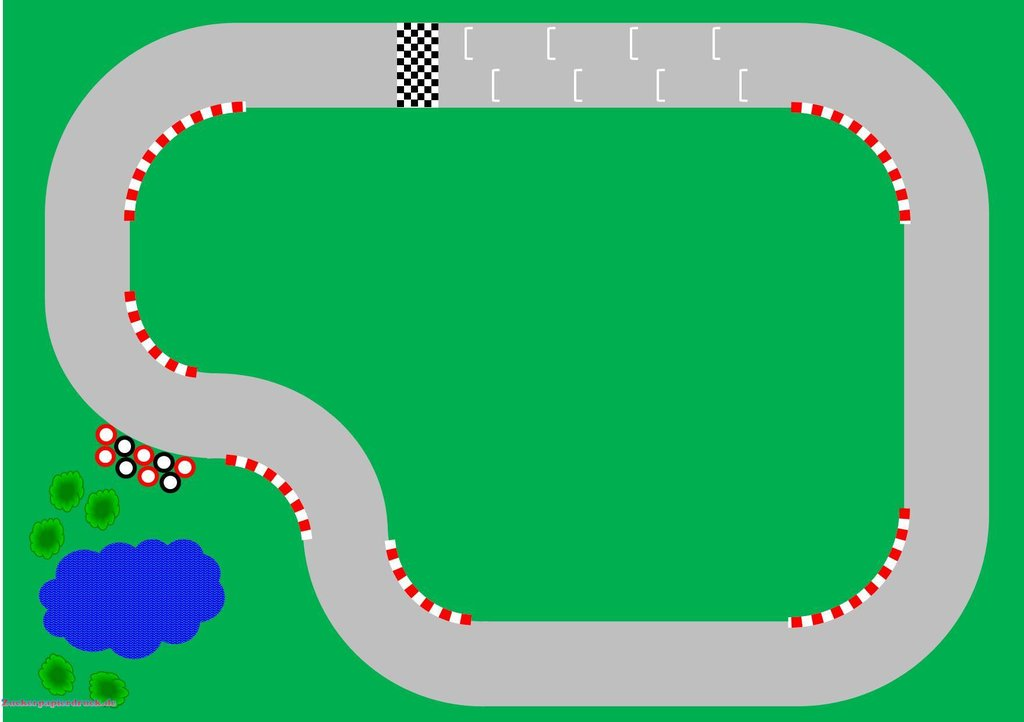
\includegraphics{../Bilder/Rennstrecke}
				\end{center}
				\caption{Erste Version der Rennstrecke} 
			\end{figure}
			
	Ursprünglich war geplant, dass rote Linien für Linkskurven stehen, blaue für Rechtskurven und grüne Linien eine Gerade bzw. ein Ende des aktuellen Segments (z.B. Boxengasse) symbolisieren. Die Gelbe Linie symbolisiert die Boxengasse. Die Außenlinie sollte durch eine einfarbige Fläche symbolisiert werden, da dies die Rückkehr auf die Strecke bei versehentlichem Verlassen der Strecke erleichtert.
	
	\bigskip
	Nach ersten Farbsensortests und Vorüberlegungen zum Ablauf der Steuerung fiel jedoch die Entscheidung, die Farbcodierungen deutlich zu vereinfachen. Die Außenlinien der Strecke sollten durch weiße Linien (z.B. Klebeband) verdeutlicht werden. Dadurch lässt sich eine beliebige Rennstrecke einfach konstruieren, in dem die Strecke mit weißem Klebeband auf schwarzem Untergrund abgeklebt wird. Dies erschwert zwar nach versehentlichem Verlassen der Strecke die Rückkehr, ist allerdings deutlich leichter und flexibler umzusetzen und spiegelt eher die Realität wieder. Des weiteren reicht es, wenn die Kurven-Eingänge und -Ausgänge mit einer Farbe markiert werden, egal ob Links- oder Rechtskurve. Die Erkennung der Kurven erfolgt dann durch ein sogenannte Einführungsrunde, in der alle Kurven erfasst werden. Außerdem kann das Auto durch diese Linien kontrollieren, wie es momentan ausgerichtet ist.
	
		\begin{figure}[h]
		\begin{center}
					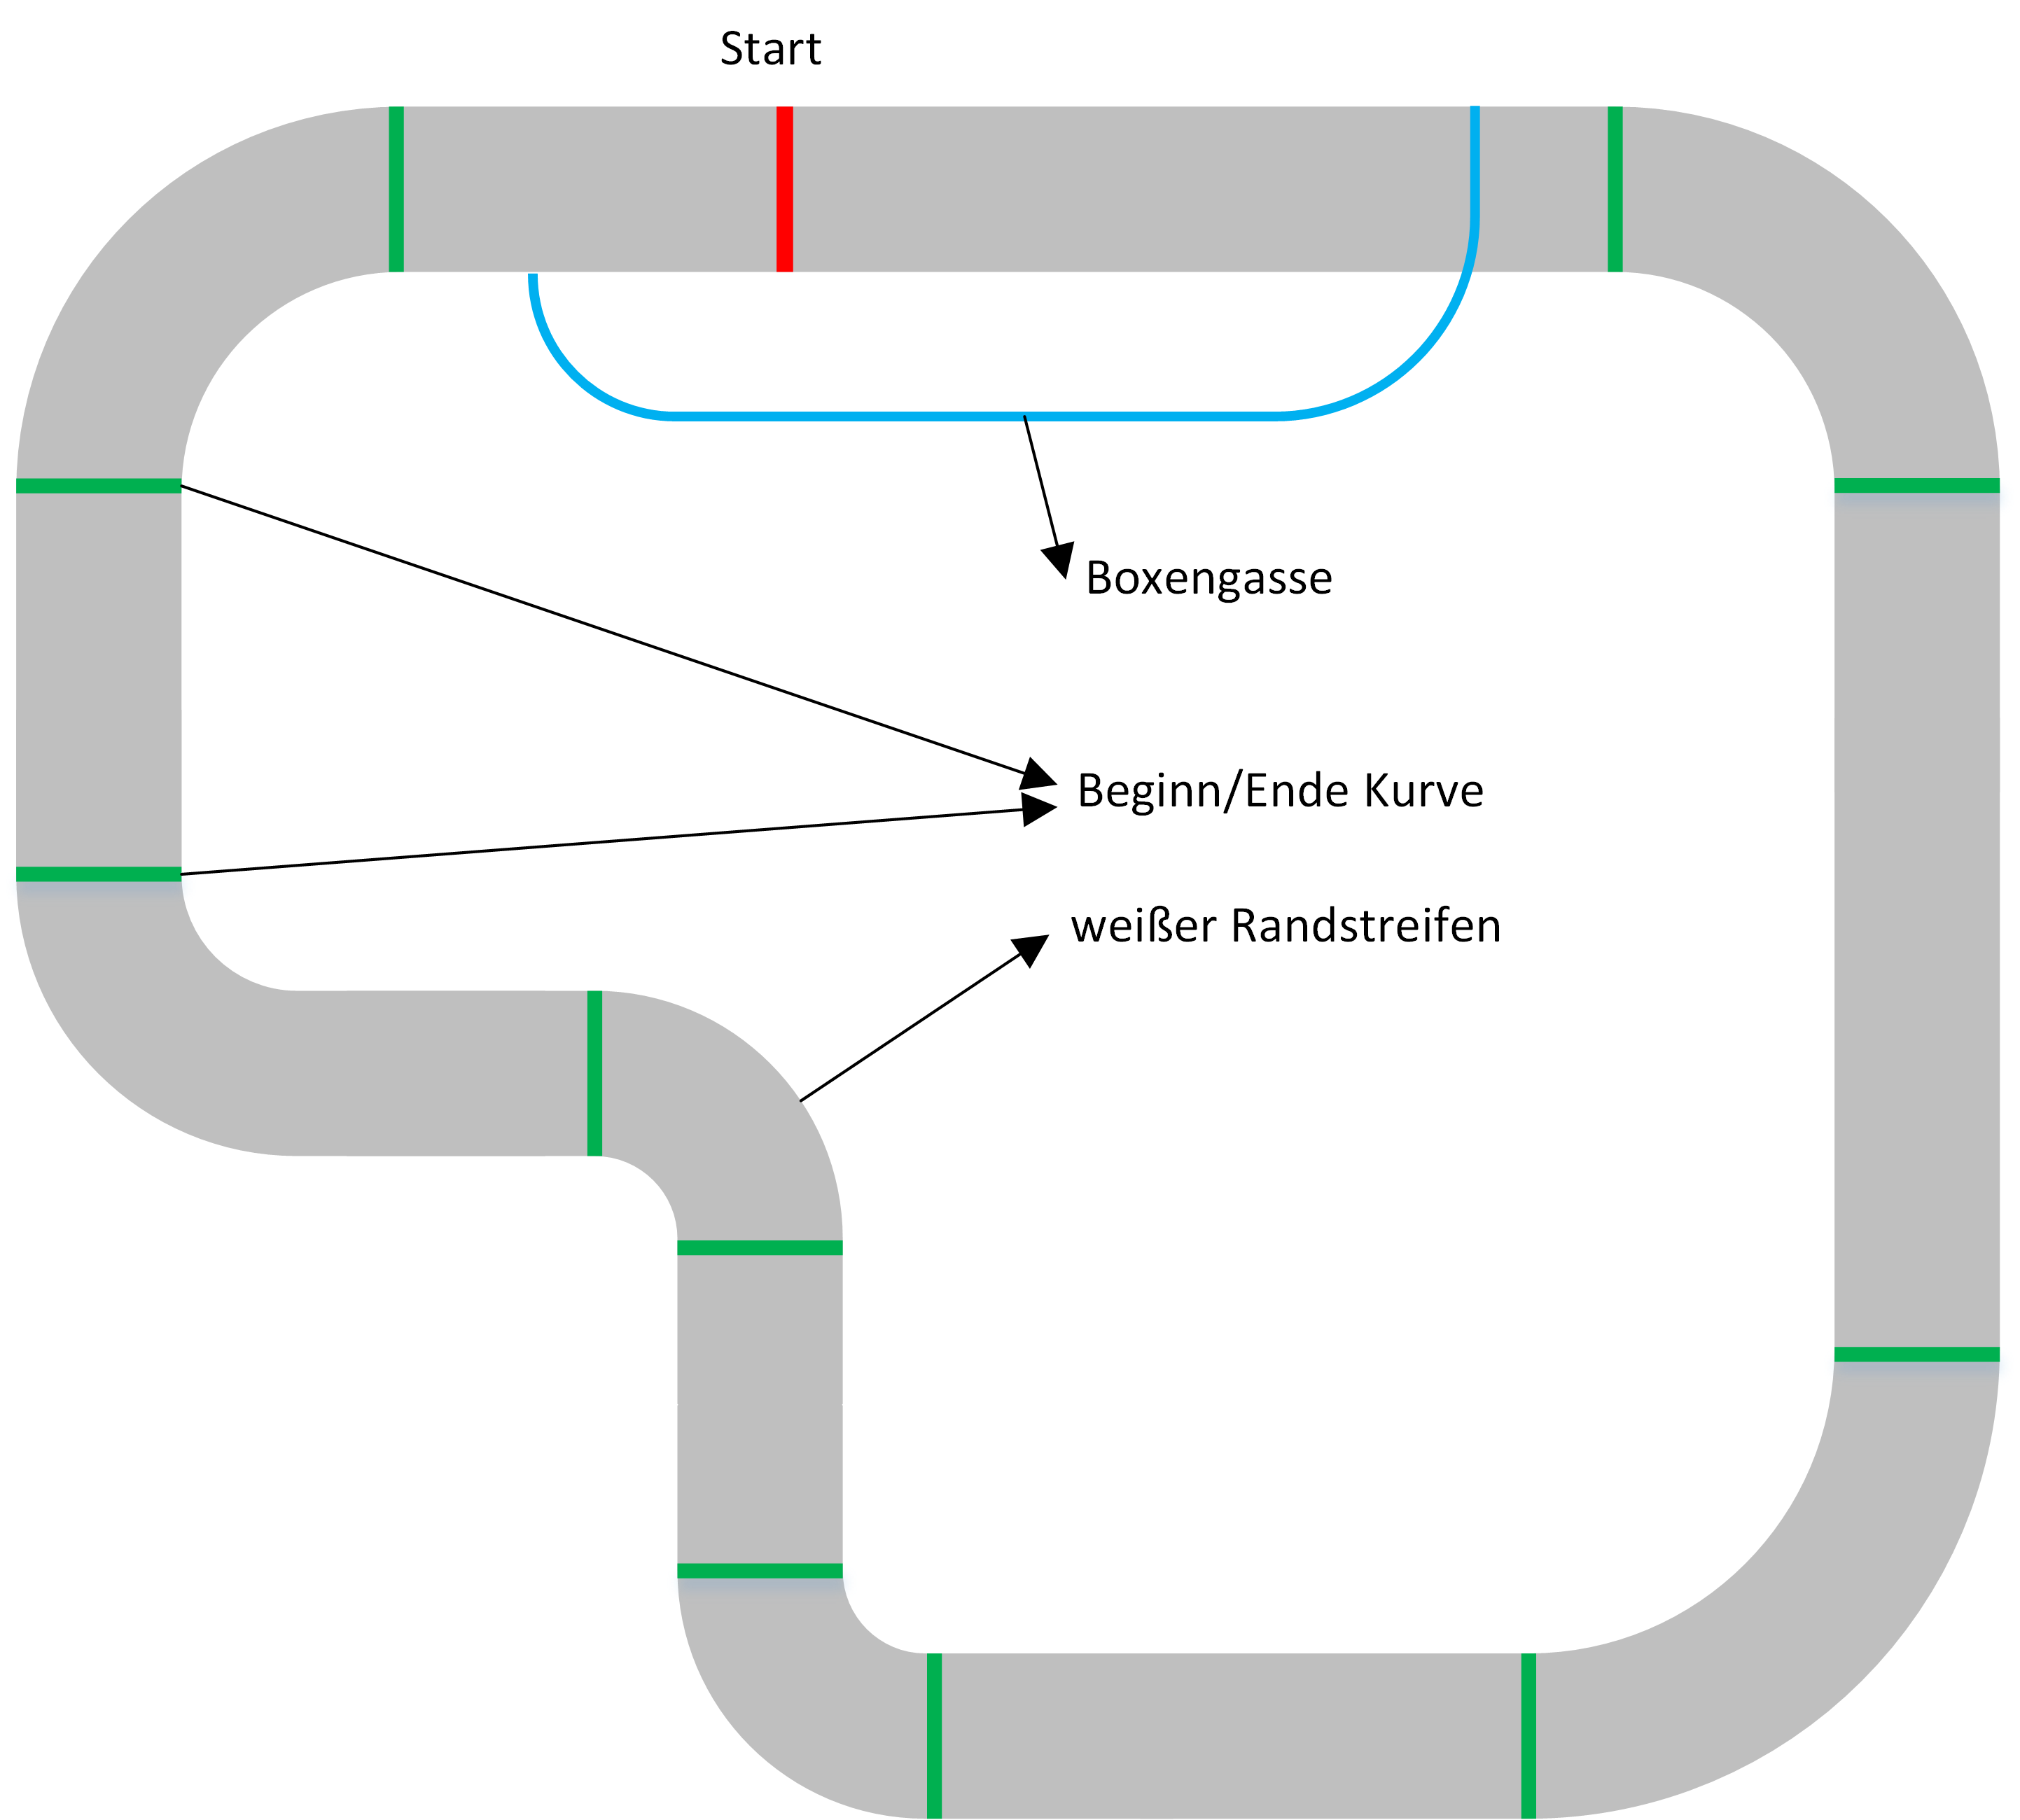
\includegraphics{../Bilder/RennstreckeBesser.png}
					\end{center}
					\caption{Verbesserte Version der Rennstrecke} 
				\end{figure}
	
	\bigskip
	 Eventuell kann später getestet werden, ob die Kurvenmarkierungen sogar ganz weggelassen werden können. Dies erfordert jedoch eine noch genauere, softwarebasierte Aufzeichnung der Strecke, was zum jetzigen Zeitpunkt noch nicht bewertet werden kann. Boxengasse sowie Start/Ziel werden weiterhin farbig markiert. Somit ergeben sich folgenden Linien:
	 
	 \bigskip
	\begin{tabular}{ l  l }
	Start/Ziel-Linie: & rot \\
	Beginn/Ende-Kurve-Lini: & grün \\ 
	Boxengasse: & blau \\
	Fahrbahnmarkierung:	& weiß \\
	\end{tabular}
	
	\newpage
	\subsection{Fahrzeuganforderungen}
		\begin{figure}[h]
					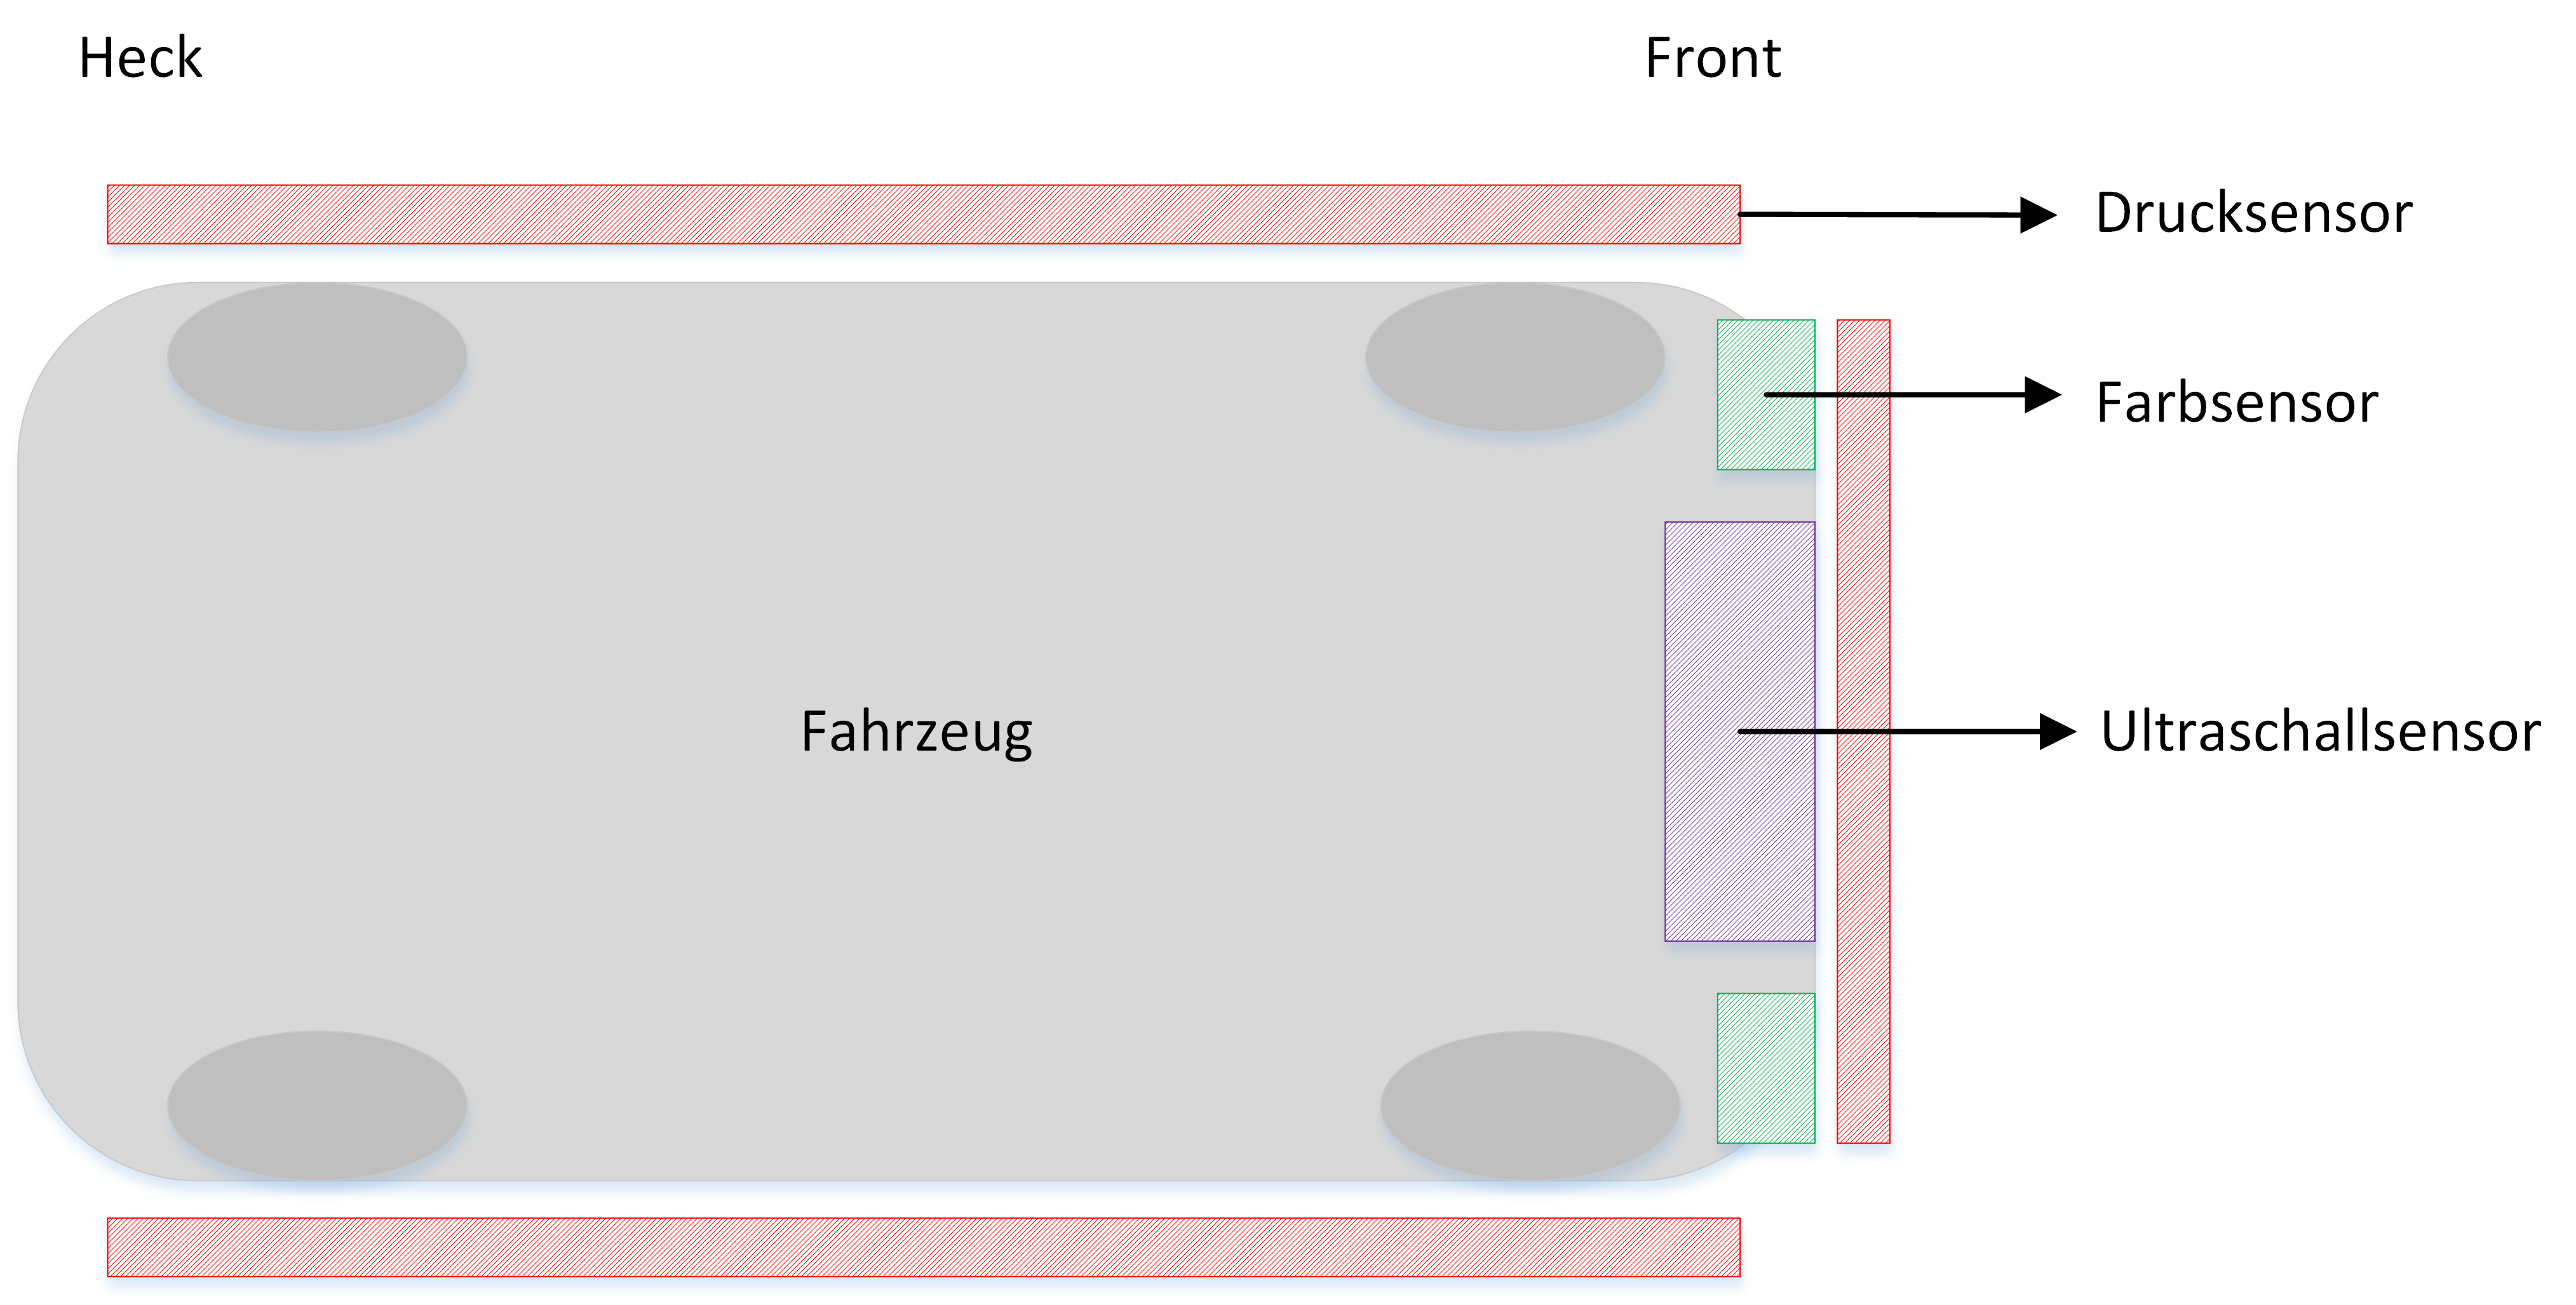
\includegraphics[scale=0.9]{../Bilder/Fahrzeug.png}
					\caption{Sensoren am Fahrzeug}
				\end{figure}
				
	Das Fahrzeug sollte an den Seiten und vorne Drucksensoren haben. Diese dienen zur Erkennung von Kollisionen und entsprechenden Reaktionen. Alternativ zu den Drucksensoren kann ein Ultraschallsensor an der Front des Fahrzeugs der Kollisionsvermeidung mit Hindernissen wie beispielsweise anderen Fahrzeugen dienen. Am Heck kann auf einen Sensor verzichtet werden, da dort im Falle einer Annäherung das auffahrende Fahrzeug die Situation erkennen würde. 
	
	\newpage
	\subsection{Aktivitätsdiagramm}
	
		\begin{figure}[h]
			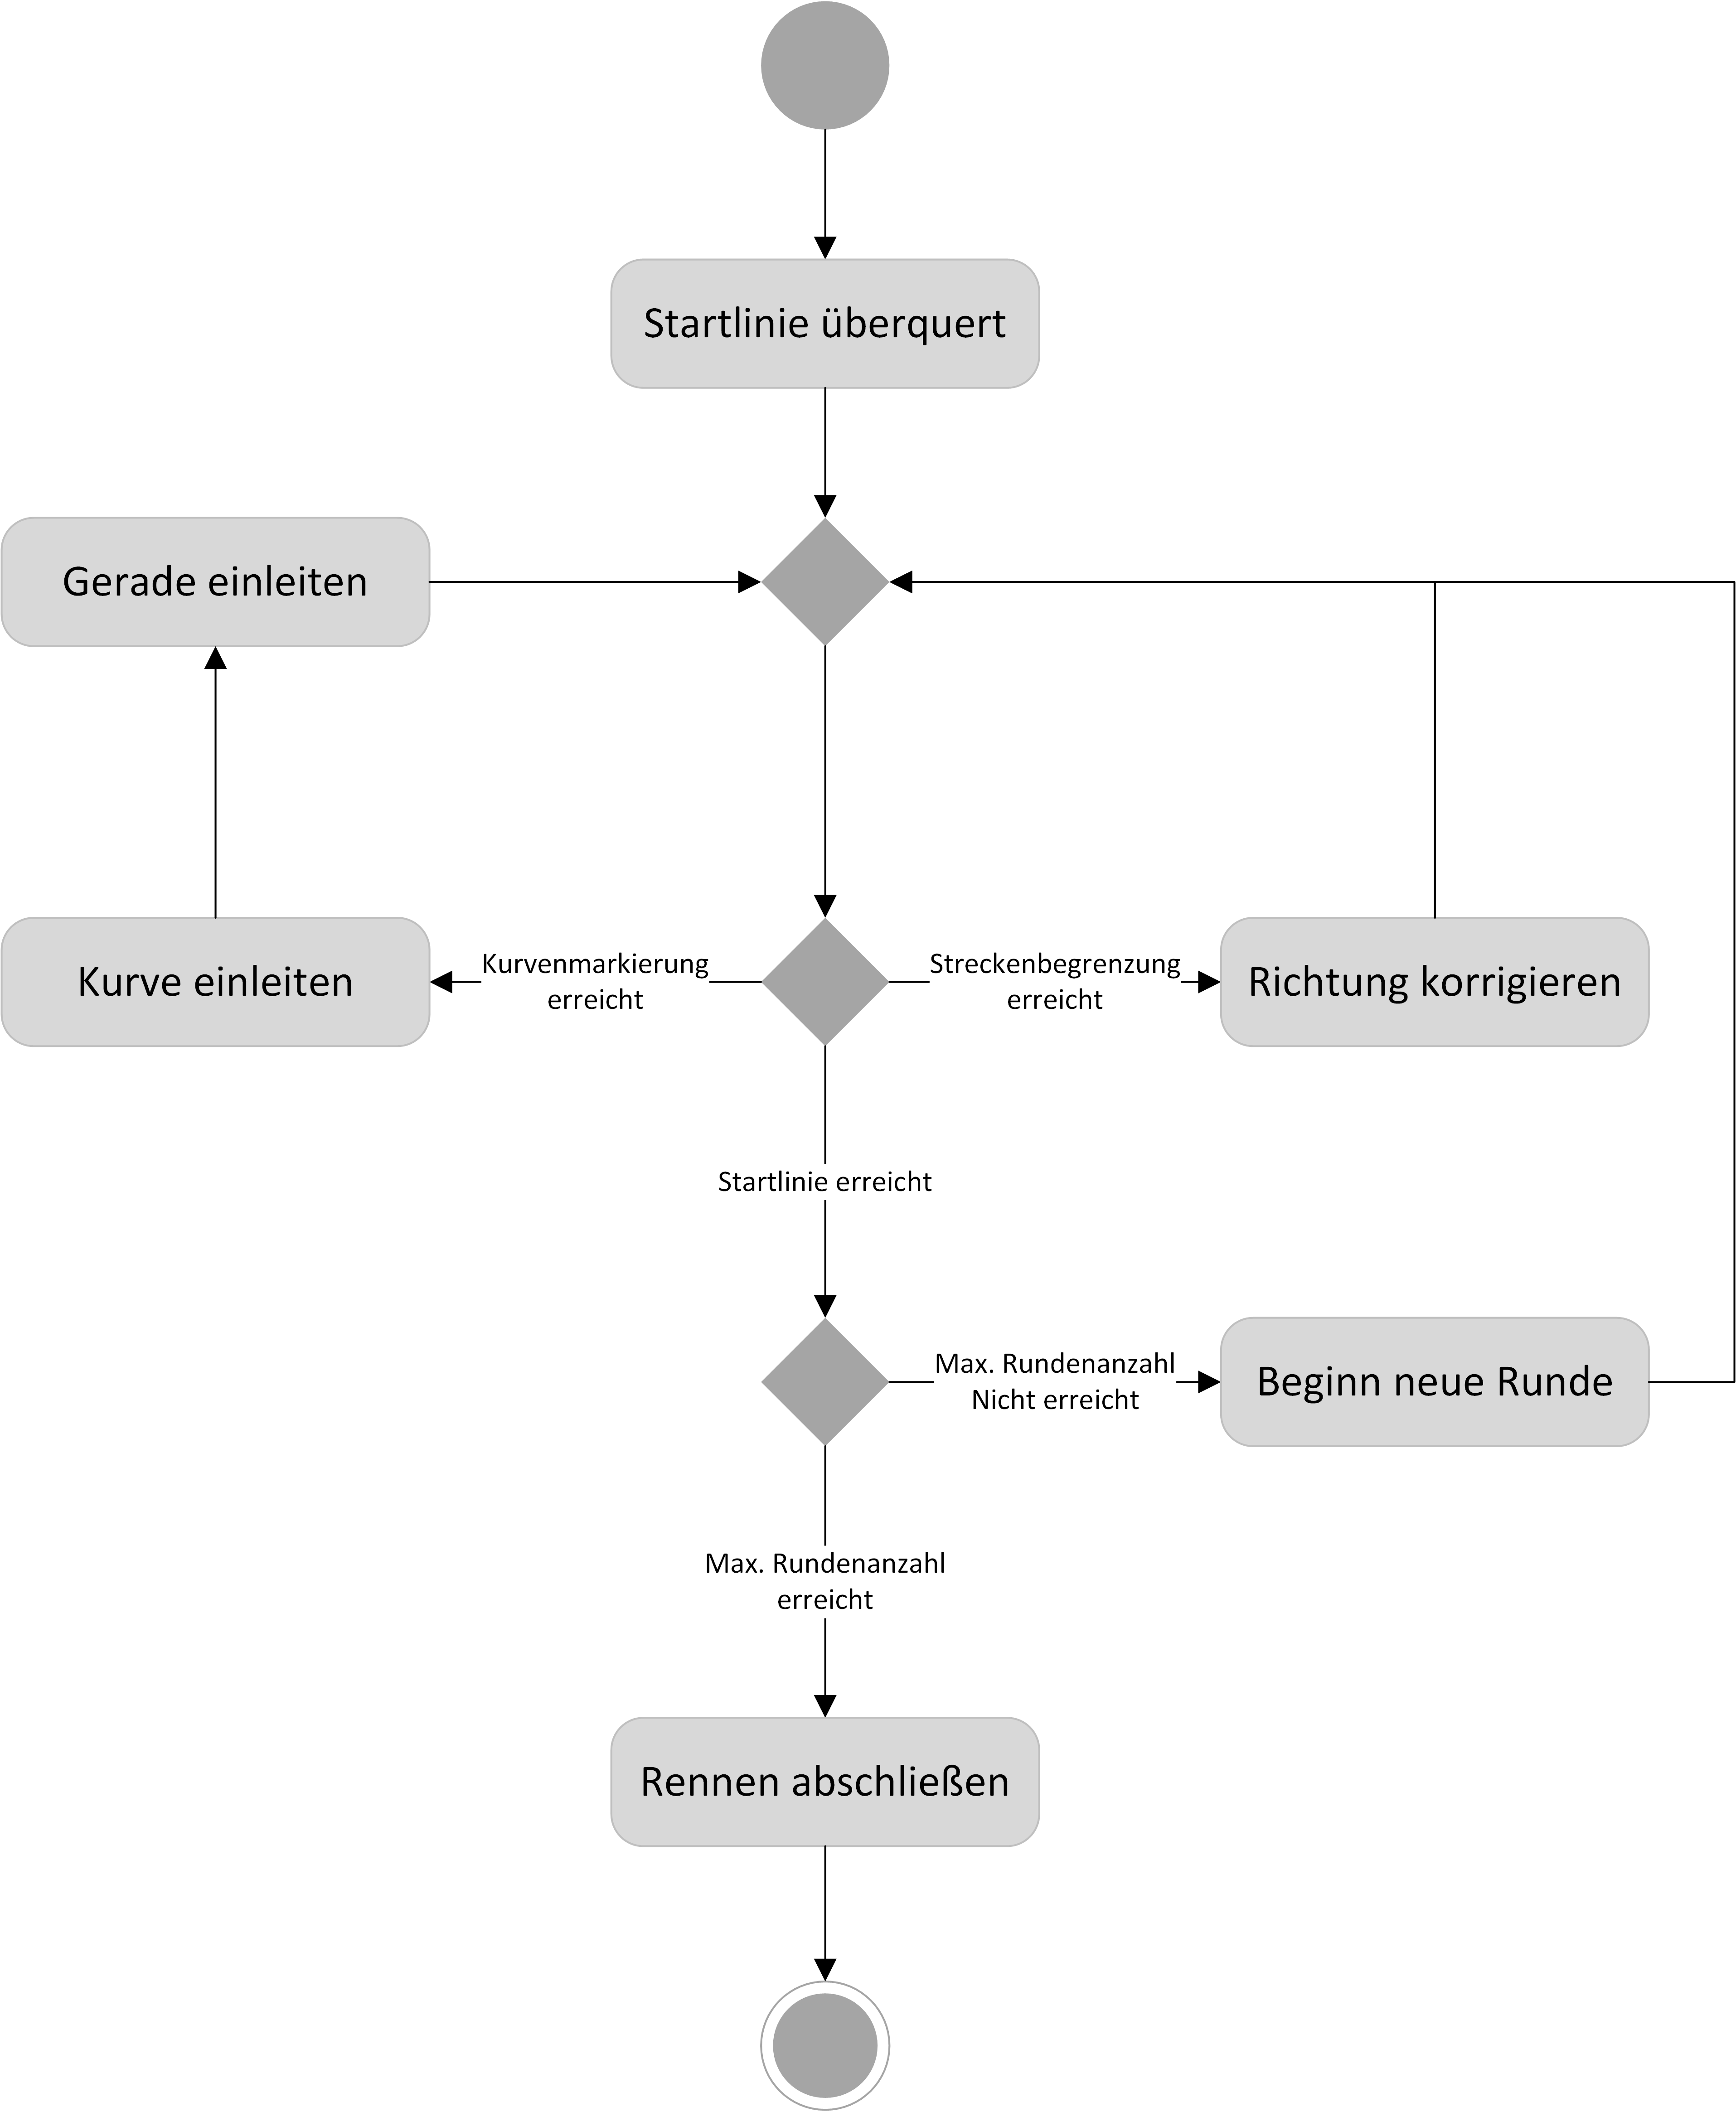
\includegraphics[scale=0.9]{../Bilder/Aktivitaetsdiagramm.png}
			\newline
			\caption{Aktivitätsdiagramm}
		\end{figure}
		
	\newpage
	\subsection{Software-Architektur}
	Die fünf High-Level-Requirements werden jeweils durch ein eigenes Package abgebildet. Der Kern des Projekts, \textit{HLR-1}, stellt das autonome Befahren der Rennstrecke dar. Die anderen vier High-Level Requirements sind Erweiterungspackages, die je nach zeitlicher Entwicklung zusätzlich implementiert werden können.
	
	\begin{figure}[h]
				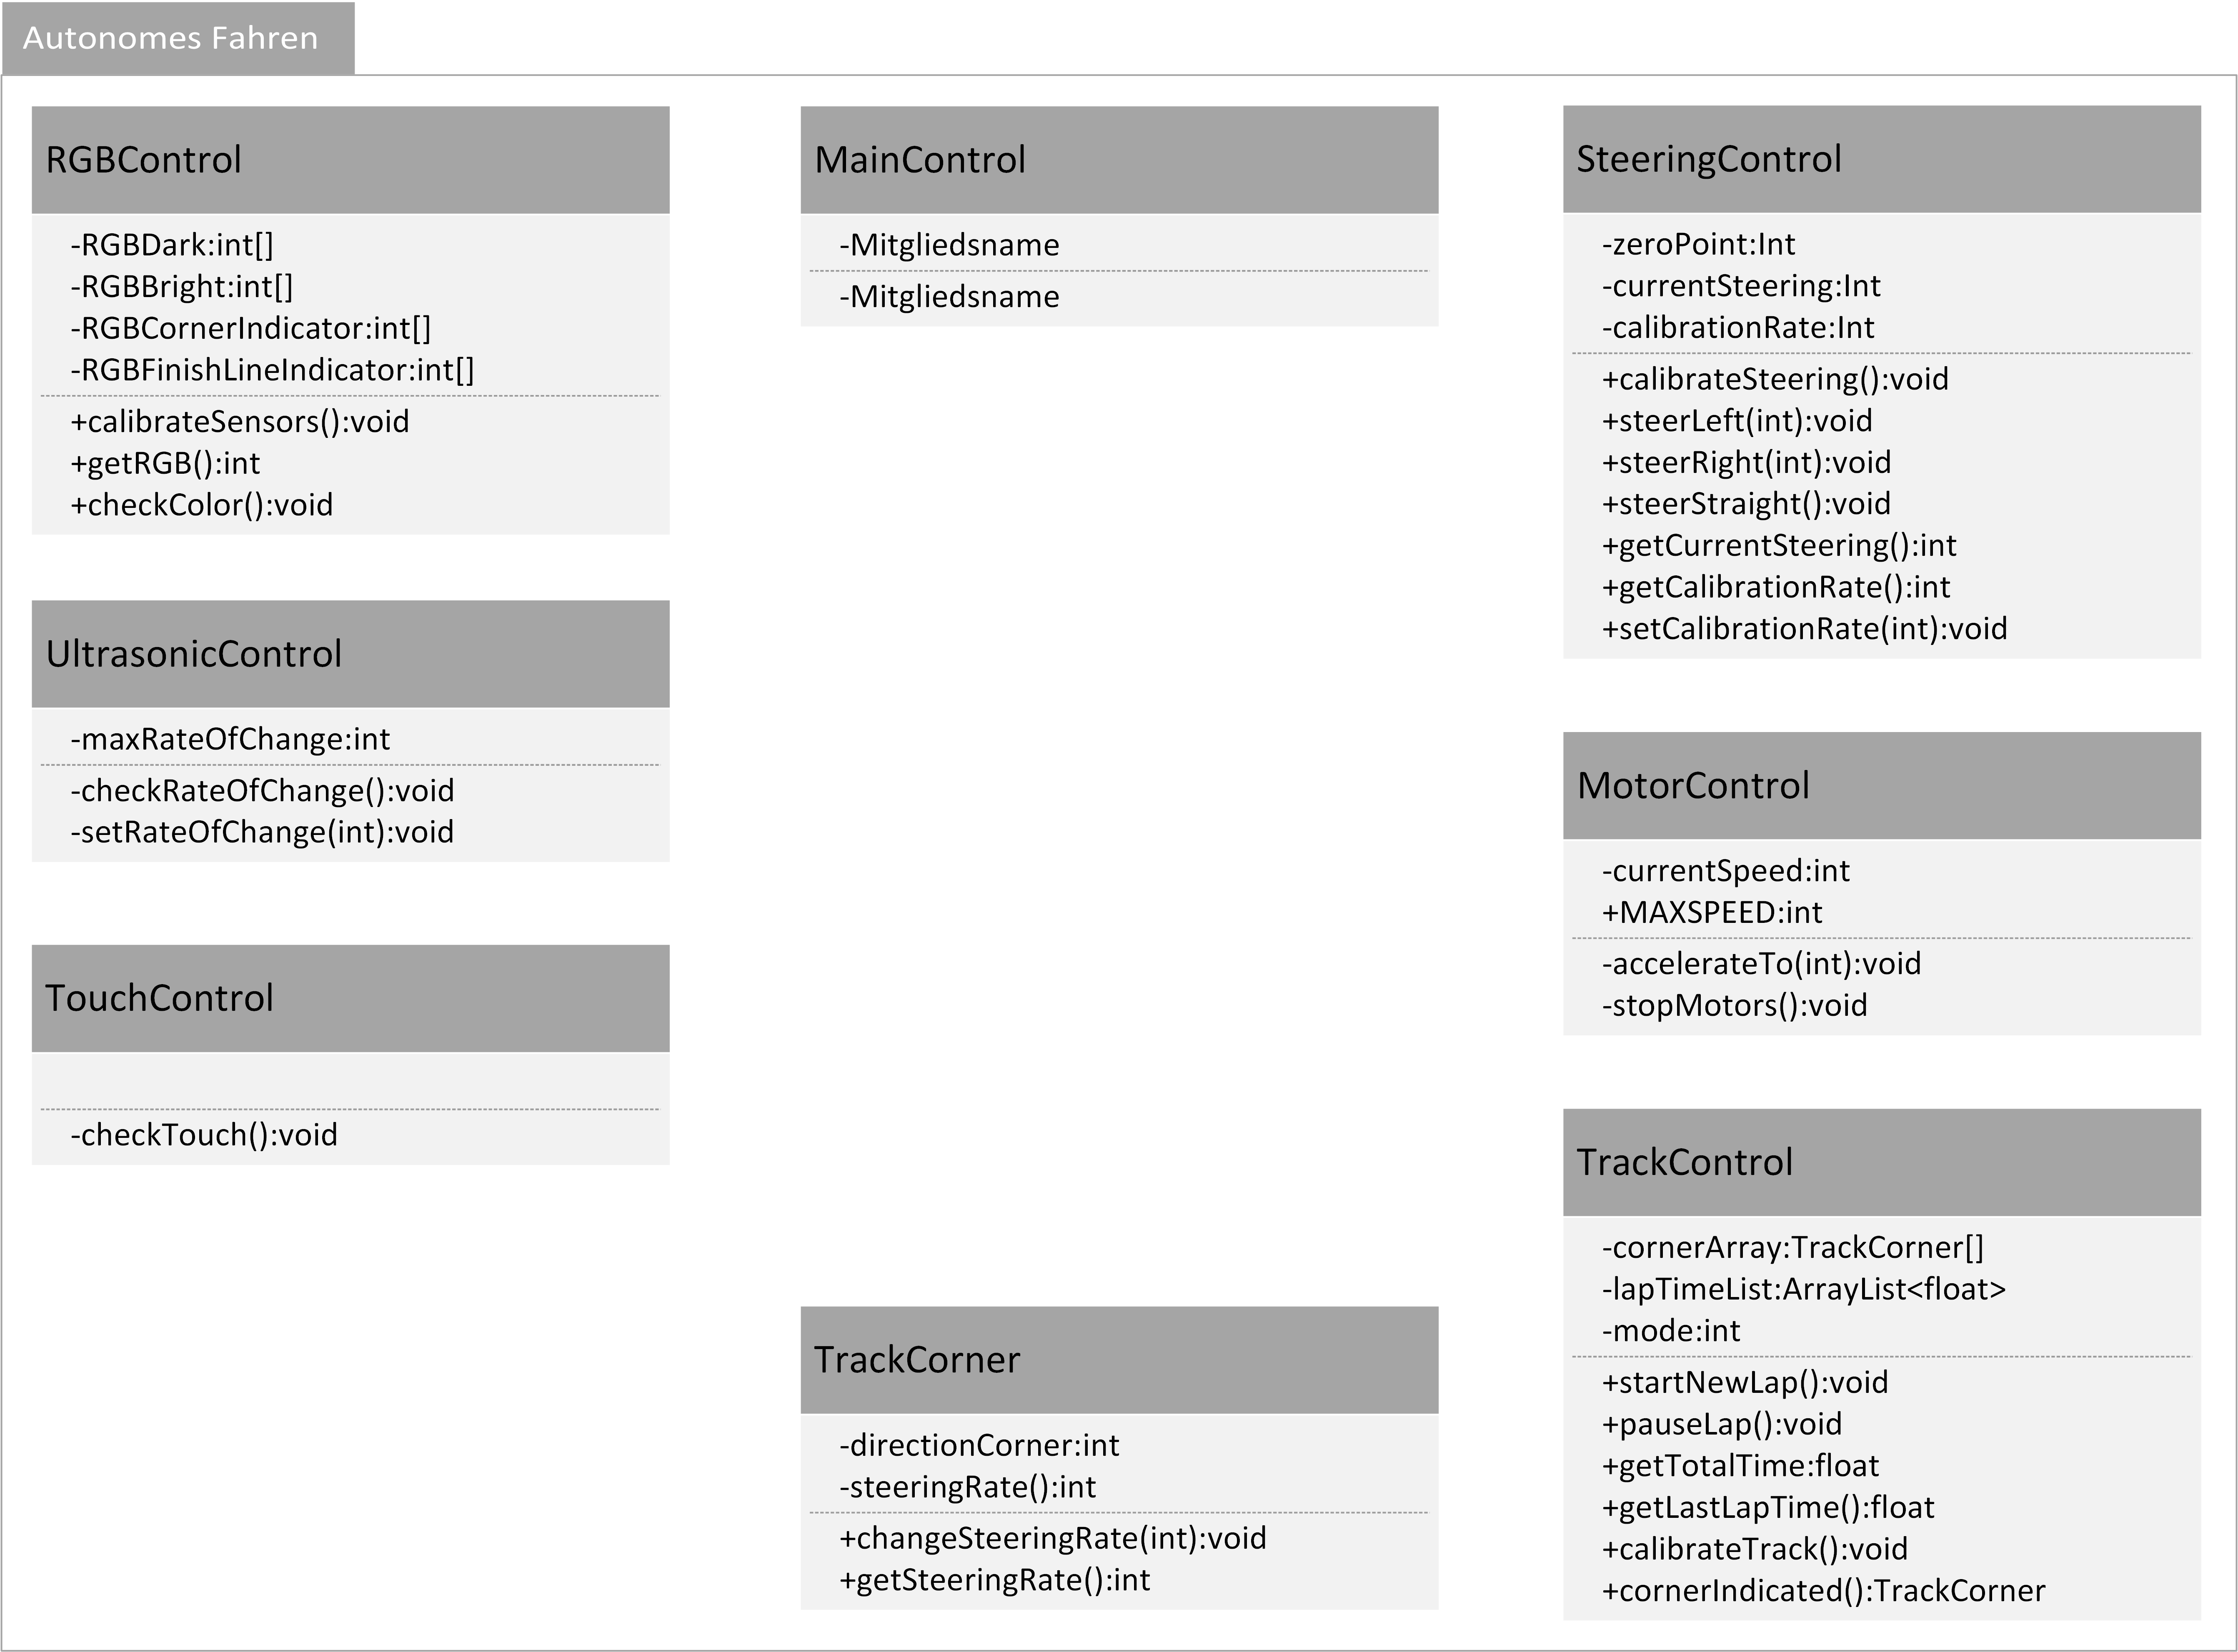
\includegraphics[scale=0.7]{../Bilder/Klassendiagramm.png}
				\caption{Klassendiagramm}
			\end{figure}
	Das Package\textit{ Autonomes Fahren} besteht aus einer Hauptklasse \textit{MainControl}, die Sensorik und Aktorik kombiniert und in Echtzeit das Auto steuert. Sie greift auf einige Nebenklassen zu, die zum Einen für die Steuerung der Motoren zuständig sind, und zum Anderen die Sensoren auswerten. Dadurch lässt sich der Ablauf deutlich vereinfachen und es ist möglich, einzelne Klassen auszutauschen (z.B. die Lenkung) ohne den gesamten Ablauf zu ändern. Damit besteht sogar die Möglichkeit, Autos unterschiedlicher Bauart (die den Spezifikationen entsprechen) zu steuern. 
	
	\bigskip
	Darüber hinaus gibt es eine Klasse, die die Rennstrecke verwaltet. Sie zeichnet in der Einführungsrunde die gefahrene Strecke möglichst genau auf. Auf diese Streckenübersicht greift die \textit{MainControl} im anschließenden Rennen zu. In Kombination mit den Sensordaten wird die Streckenübersicht auch während dem Rennen ständig verbessert um so eine möglichst optimale Linie zu fahren.
	
	\newpage
	
	\section{Erste Umsetzungsphase}
	\subsection{Entwicklungsentscheidungen}
	Bei dem System handelt es sich um ein Echtzeitsystem, das jedoch keine harten Deadlines einhalten muss. Generell charakterisiert ein Echtzeitsystem das rechtzeitige Eintreffen eines Ergebnisses. Im konkreten Fall muss das Fahrzeug auf die Streckeneigenschaften reagieren und  Kollisionen mit anderen Fahrzeugen vermeiden oder gewollt herbeiführen. Daher sind gewisse Zeitfenster in der Streckenkalkulation einzuhalten, sodass das Fahrzeug nicht von der Fahrbahn abweicht. Zudem sollte  bei der Erkennung einer möglichen Kollision das Signal zu einem bestimmten Zeitpunkt in der Recheneinheit ankommen, sodass es dort abgefangen und darauf reagiert werden kann. Diese Bedingungen sind mit keinen harten Echtzeitbedingungen verbunden, d.h. bei Nichteinhalten wird kein großer Schaden verursacht.
	Diese Betrachtungen lassen auf den Einsatz einer Programmiersprache schließen, die keine harten Echtzeitbedingungen unterstützen muss. Java reicht für den Anwendungsfall völlig aus.
	
	\bigskip
	Als Entwicklungsumgebung kommt Eclipse Mars zum Einsatz. Dabei ist zu beachten, dass die 32bit Version von Eclipse, JDR und JDK Vorraussetzung für ein erfolgreiches Übertragen auf den NXT ist. 
	
	\bigskip
	Für die Erstellung eine umfassende Dokumentation wird der Web-Editor GoogleDocuments genutzt, sodass das gesamte Team parallel an den Dokumenten arbeiten kann. Als Versionsverwaltungstool der Software soll GitHub zum Einsatz kommen.
	
	\newpage
	\subsection{Sensortests}
	\subsubsection{Farbsensor}
	Als Farbsensoren werden RGB-Sensoren verwendet. Da die Farbe abhängig vom einfallenden Licht und der Entfernung des Sensors zum Untergrund ist, haben wir speziell auf den konkreten Anwendungsfall abgestimmte Sensortests vorgenommen. Vor dem Start eines Rennens soll auf Basis der gemessenen Werte eine Sensor-Kalibrierung vorgenommen werden, sodass sich die Software im Fahrzeug auf die aktuell herrschenden Lichtbedingungen einstellen kann.  
	
	\bigskip
	Eine erste Messreihe ergab folgende Rot-, Grün- und Blauwerte für die aufgelisteten farbigen Untergründe:
	
	\begin{tabular}{ l | l | l | l }
		\textbf{Farbe des Untergrunds} & \textbf{Blauwert} & \textbf{Grünwert} & \textbf{Rotwert} \\ \hline
		rot (Trennblatt) & 101 & 920 & 260\\
		grün (Trennblatt) & 126 & 193 & 111 \\
		gelb (Trennblatt) & 185 & 278 & 260 \\
		blau (Trennblatt) & 250 & 202 & 125 \\
		schwarz (Schaumstoffplatte) & 350 & 460 & 598 \\
		weiß (Kreppband) & 220 & 240 & 250 \\
	\end{tabular}
	
	\bigskip
	Wie man anhand der Messreihe sehen kann, können einige Werte nicht korrekt sein. Da bei erneutem Messen jedoch ähnliche Werte auftraten, haben wir uns für eine Umgehung des Problems durch eine Softwarelösung entschieden.
	Eine genauere Betrachtung der Werte lässt den Schluss zu, dass alle Werte zwischen 255 und 300 den Wert 255 annehmen sollten. Alle Werte, die größer als 300 sind, sollten den Wert 0 annehmen. Durch eine solche Umsetzung werden die Farben entsprechend richtig dargestellt:
	
	\bigskip
	
		\begin{tabular}{ l | l | l | l }
			\textbf{Farbe des Untergrunds} & \textbf{Blauwert{\tiny (korrigiert)}} & \textbf{Grünwert{\tiny (korr.)}} & \textbf{Rotwert{\tiny (korr.)}} \\ \hline
			rot (Trennblatt) & 101 & 0 & 255\\
			grün (Trennblatt) & 126 & 193 & 111 \\
			gelb (Trennblatt) & 185 & 255 & 255 \\
			blau (Trennblatt) & 250 & 202 & 125 \\
			schwarz (Schaumstoffplatte) & 0 & 0 & 0 \\
			weiß (Kreppband) & 220 & 240 & 250 \\
		\end{tabular}
		
	\bigskip
	Die meisten Farben lassen sich laut Testreihe relativ gut unterscheiden. Lediglich der Unterschied zwischen gelb und weiß (in dem Fall Kreppband) ist sehr gering. Deshalb werden gelbe Linien nicht verwendet (siehe Abschnitt\textit{ Streckengestaltung}).
	
	\subsubsection{Drucksensor}
	Die Drucksensoren dienen der frühzeitigen Kollisionserkennung. Anhand eines Drucktests stellte sich heraus, dass der Sensor ein Hindernis erst bei vollständig eingedrücktem Sensorfeld erkennt. Leichter Druck löst keine Zustandsänderung aus. Dies könnte ein Problem bei der späteren Umsetzung darstellen, da ein spezieller Aufbau nötig wird, um eine bevorstehende Kollision zu erkennen, bevor sie tatsächlich eintritt. 
	
	\subsubsection{Ultraschallsensor}
	Der Ultraschallsensor dient der Hinderniserkennung. Es soll die gesamte vor dem Fahrzeug liegende Fläche abgedeckt werden, sodass bei einem Rennen mit mehreren Fahrzeugen Kollisionen vermieden werden können. \\
	
	\begin{figure}[h]
		\begin{center}
			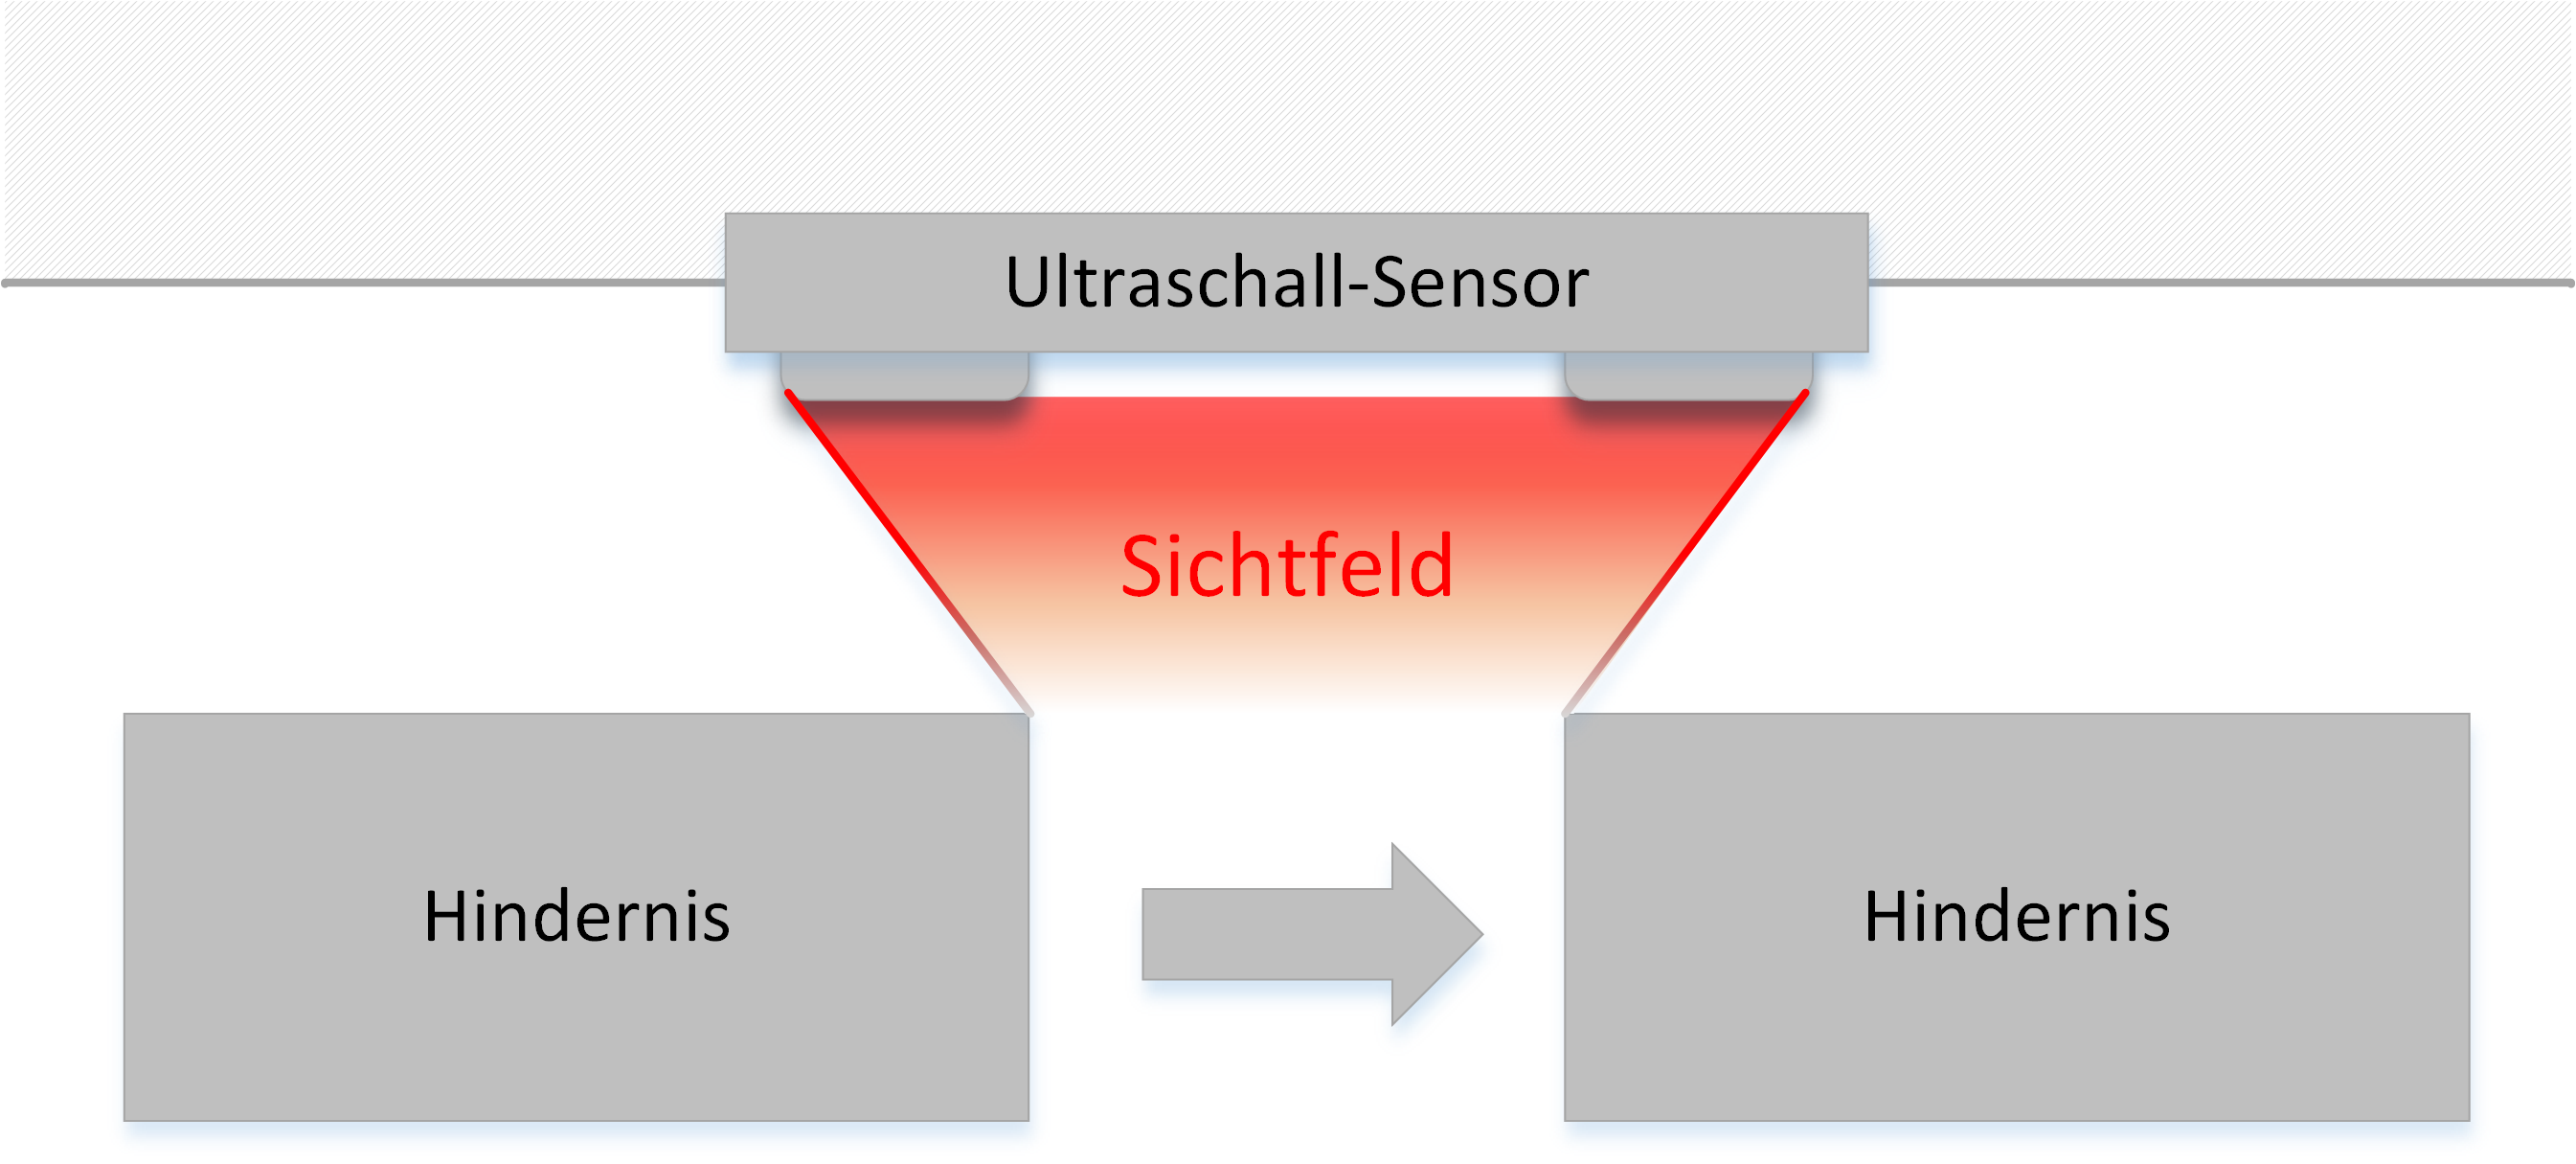
\includegraphics{../Bilder/Ultraschallsensor.png}
		\end{center}
		\caption{Sichtfeld eines Ultraschallsensors}
	\end{figure}
	
	Mit Hilfe eines etwa 4 cm hohen Hindernisses wurde das Sichtfeld des Ultraschallsensors ermittelt. Dabei wurde der Sensor etwa auf der Höhe befestigt, auf der er sich auch später im Fahrzeug befinden soll. Durch langsames Vorbeischieben des Hindernisses parallel zum Sensor konnte der Bereich festgestellt werden, innerhalb dem der Sensor das Hindernis erkennt. Die vom Sensor erkannten Werte wurden auf dem Display des NXT angezeigt. Ein schlagartiger Wechsel auf eine bedeutend kleinere Zahl war ein Indiz für ein Hindernis. 
	
	\bigskip
	Bei diesem Versuchsaufbau stellte sich heraus, dass das Sichtfeld des Ultraschall-Sensors recht eingeschränkt ist und nur einen kleinen Bereich der davorliegenden Fläche wahrgenommen wird. Ein einzelner Ultraschall-Sensor ist für die Hinderniserkennung eines Fahrzeugs somit nicht geeignet.
	
	\newpage
	\section{Reflexion des ersten Standes}
	Wir begannen mit dem Projekt im Oktober 2015. Die Entscheidung des Themas fiel recht schnell, wir waren uns einig, dass es sich als Studienarbeitsthema hervorragend eignet. Es kann beliebig erweitert werden und bietet eine Reihe an Möglichkeiten, Erlerntes zu vertiefen und Neues zu lernen. Während die Grundsteuerung der Fahrzeuge recht schnell umgesetzt und ein erster Stand bereits nach wenigen Wochen erreicht war, erfordern komplexeren Überlegungen eine genaue Planung. Daher haben wir uns einige Zeit mit einem Entwurf der Software-Architektur beschäftigt, um diese möglichst einfach erweiterbar zu gestalten. Auf Basis des aktuellen Projektplans haben wir fehlende Bauteile bestellt, die auch bereits eingetroffen sind. 
	
	\bigskip
	Der Umstand, dass für erfolgreiches Übertragen auf den NXT spezielle Versionen von Java und Eclipse nötig sind, brachte einiges an Arbeitsaufwand mit sich. Bis die Entwicklungsumgebung bei allen Teammitgliedern wie vorgesehen funktionierte, dauerte es einige Wochen. Das schränkte den Arbeitsfortschritt zunächst erheblich ein. 
	
	\bigskip
	Bisher haben wir uns etwa wöchentlich einmal für ein paar Stunden zusammengesetzt und an dem Projekt weitergearbeitet. Die Dokumentation erfolgt außerhalb dieser Zeiten online über ein geteiltes Dokument, das jedes Teammitglied bearbeiten kann. Das Projekt bietet die Möglichkeit, ab einem gewissen Stand einzeln an den Fahrzeugen weiterzuarbeiten. Denn Ziel sind mehrere Fahrzeuge, die gegeneinander antreten. So kann auch innerhalb des Teams ein Wettbewerb stattfinden, wer das beste Fahrzeug baut und programmiert. 
	Generell funktioniert die Teamarbeit in unserem Projekt sehr gut, da sich jeder für das Projekt interessiert und verantwortlich fühlt.
	
	\bigskip
	Die genaue Verteilung der Sensoren auf dem Fahrzeug (siehe Kapitel \textit{Fahrzeuganforderungen}) wird aktuell diskutiert. Unter anderem steht die Frage der Verwendung eines Multiplexers im Raum, um so mehr Sensoren an den NXT anschließen und in der Software verwenden zu können. 
	
	\newpage
	\section{Projektplan zum weiteren Vorgehen}
	
		\begin{figure}[h]
			\begin{center}
				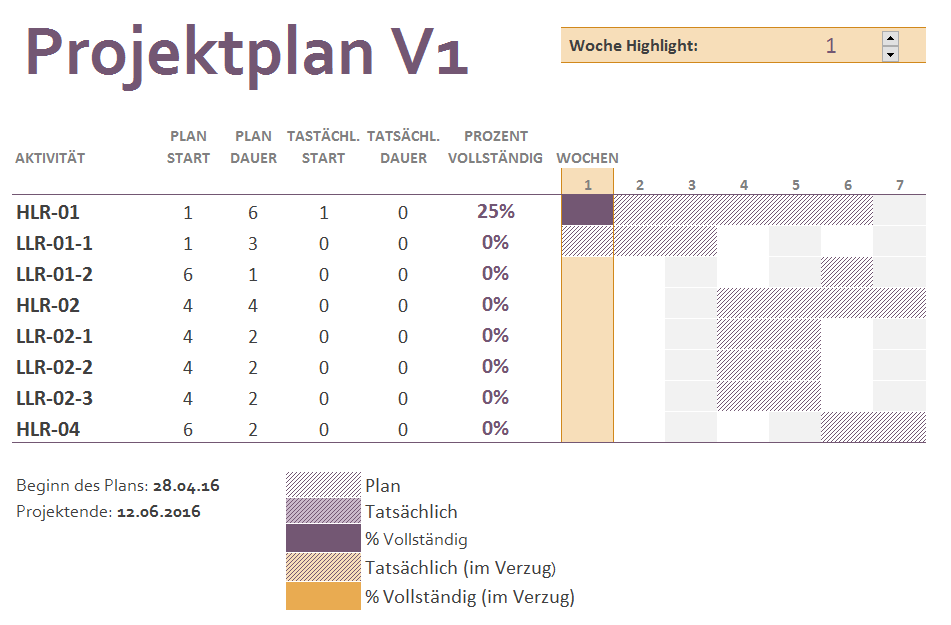
\includegraphics[scale=0.8]{../Bilder/PlanV1.png}
			\end{center}
			\caption{Projektplan Version 1}
		\end{figure}
		
	Die Aktivitäten im Projektplan beziehen sich auf die in Kapitel~\ref{kap:reqs} beschriebenen Software-Requirements. Zum Zeitpunkt der Erstellung des Projektplans (28.04.16) existiert ein erster Ansatz der Motorsteuerung. Daher rühren die 25\% in der Spalte "Prozent vollständig" bei HLR-01. Es wurde ein prototypisches Modell des Fahrzeugs entworfen und dieses bereits in der Anfangsphase des Projektes weiterentwickelt. Ein funktionsfähiges Fahrzeig ist somit Grundlage des Projektplans, ohne das die Umsetzung der Software-Anforderungen nicht möglich wäre. 
	
	\bigskip
	In Kapitel~\ref{kap:reqs} werden insgesamt sechs Highlevel-Software-Anforderungen beschrieben. In Anbetracht der Komplexität der in HLR-01 bis HLR-04 umrissenen Anforderungen haben wir uns entschieden, HLR-05 und HLR-06 zunächst außen vor zu lassen. Sollte Umsetzung der Grundfunktionalitäten doch schneller als erwartet verlaufen, kann der Projektplan um die Implementierung einer Smarthone-App und deren Anbindung an die Fahrzeuge erweitert werden.
	
	\bigskip
	Geplanter Projektabschluss ist der 12.06.16. So ist genügend zeitlicher Puffer bis zum vorgegebenen Abgabeende des Projektes. 
	
	\newpage
	\section{Zweite Umsetzungsphase}
	\subsection{Fertigung der Rennstrecke}
	Als Rennstrecke dienen drei Sperrholz-Platten, die zu einer großen Platte mit den Maßen 2m x 1,80m zusammengefügt werden können. Um die Farberkennung durch die RGB-Sensoren möglichst fehlerresistent zu gestalten, wurden die Platten weiß bemalt. Als Fahrbahn dient eine speziell zugeschnittene schwarze Folie.
	
	\begin{figure}[h!]
	\centering
	\begin{subfigure}{.5\textwidth}
	  \centering
	  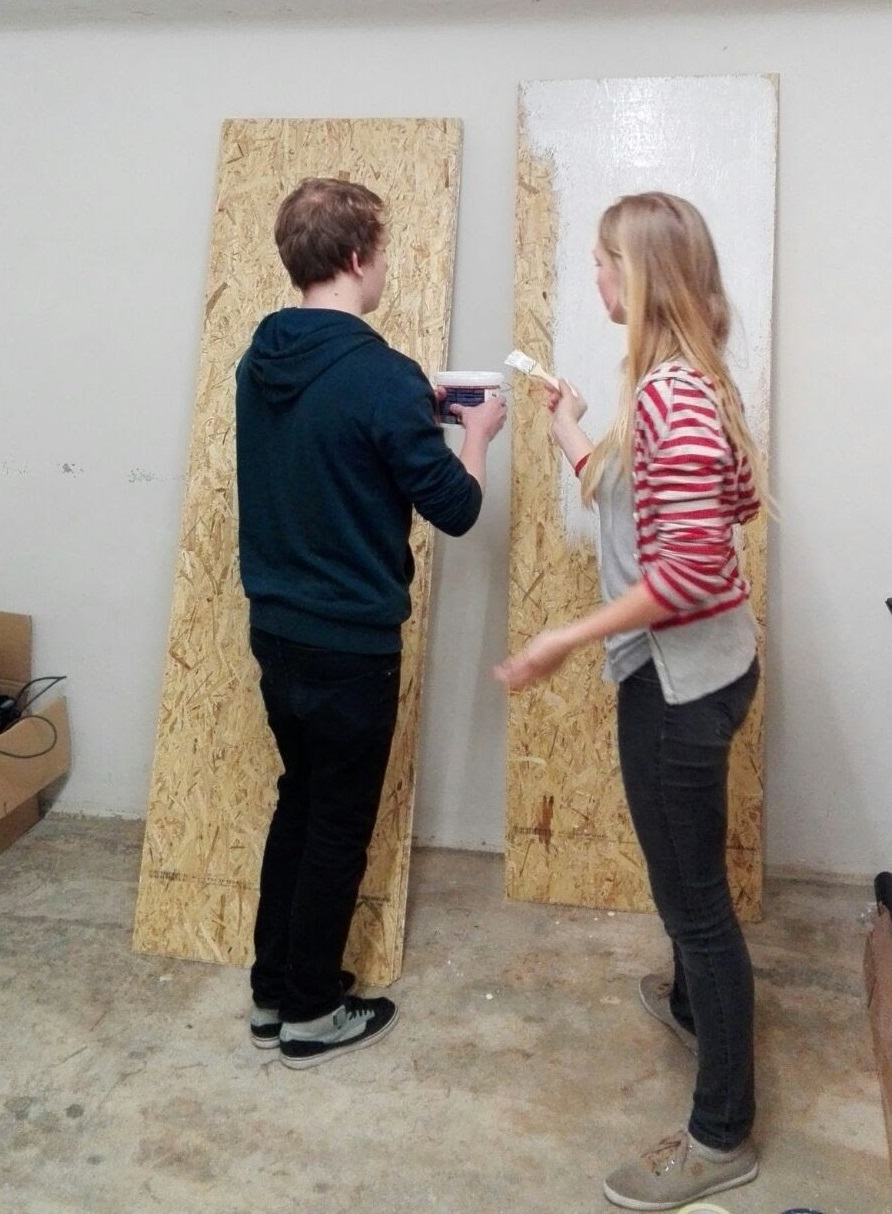
\includegraphics[width=.6\linewidth]{../Bilder/plattenmalen.jpg}
	  \label{fig:sub1}
	\end{subfigure}%
	\begin{subfigure}{.5\textwidth}
	  \centering
	  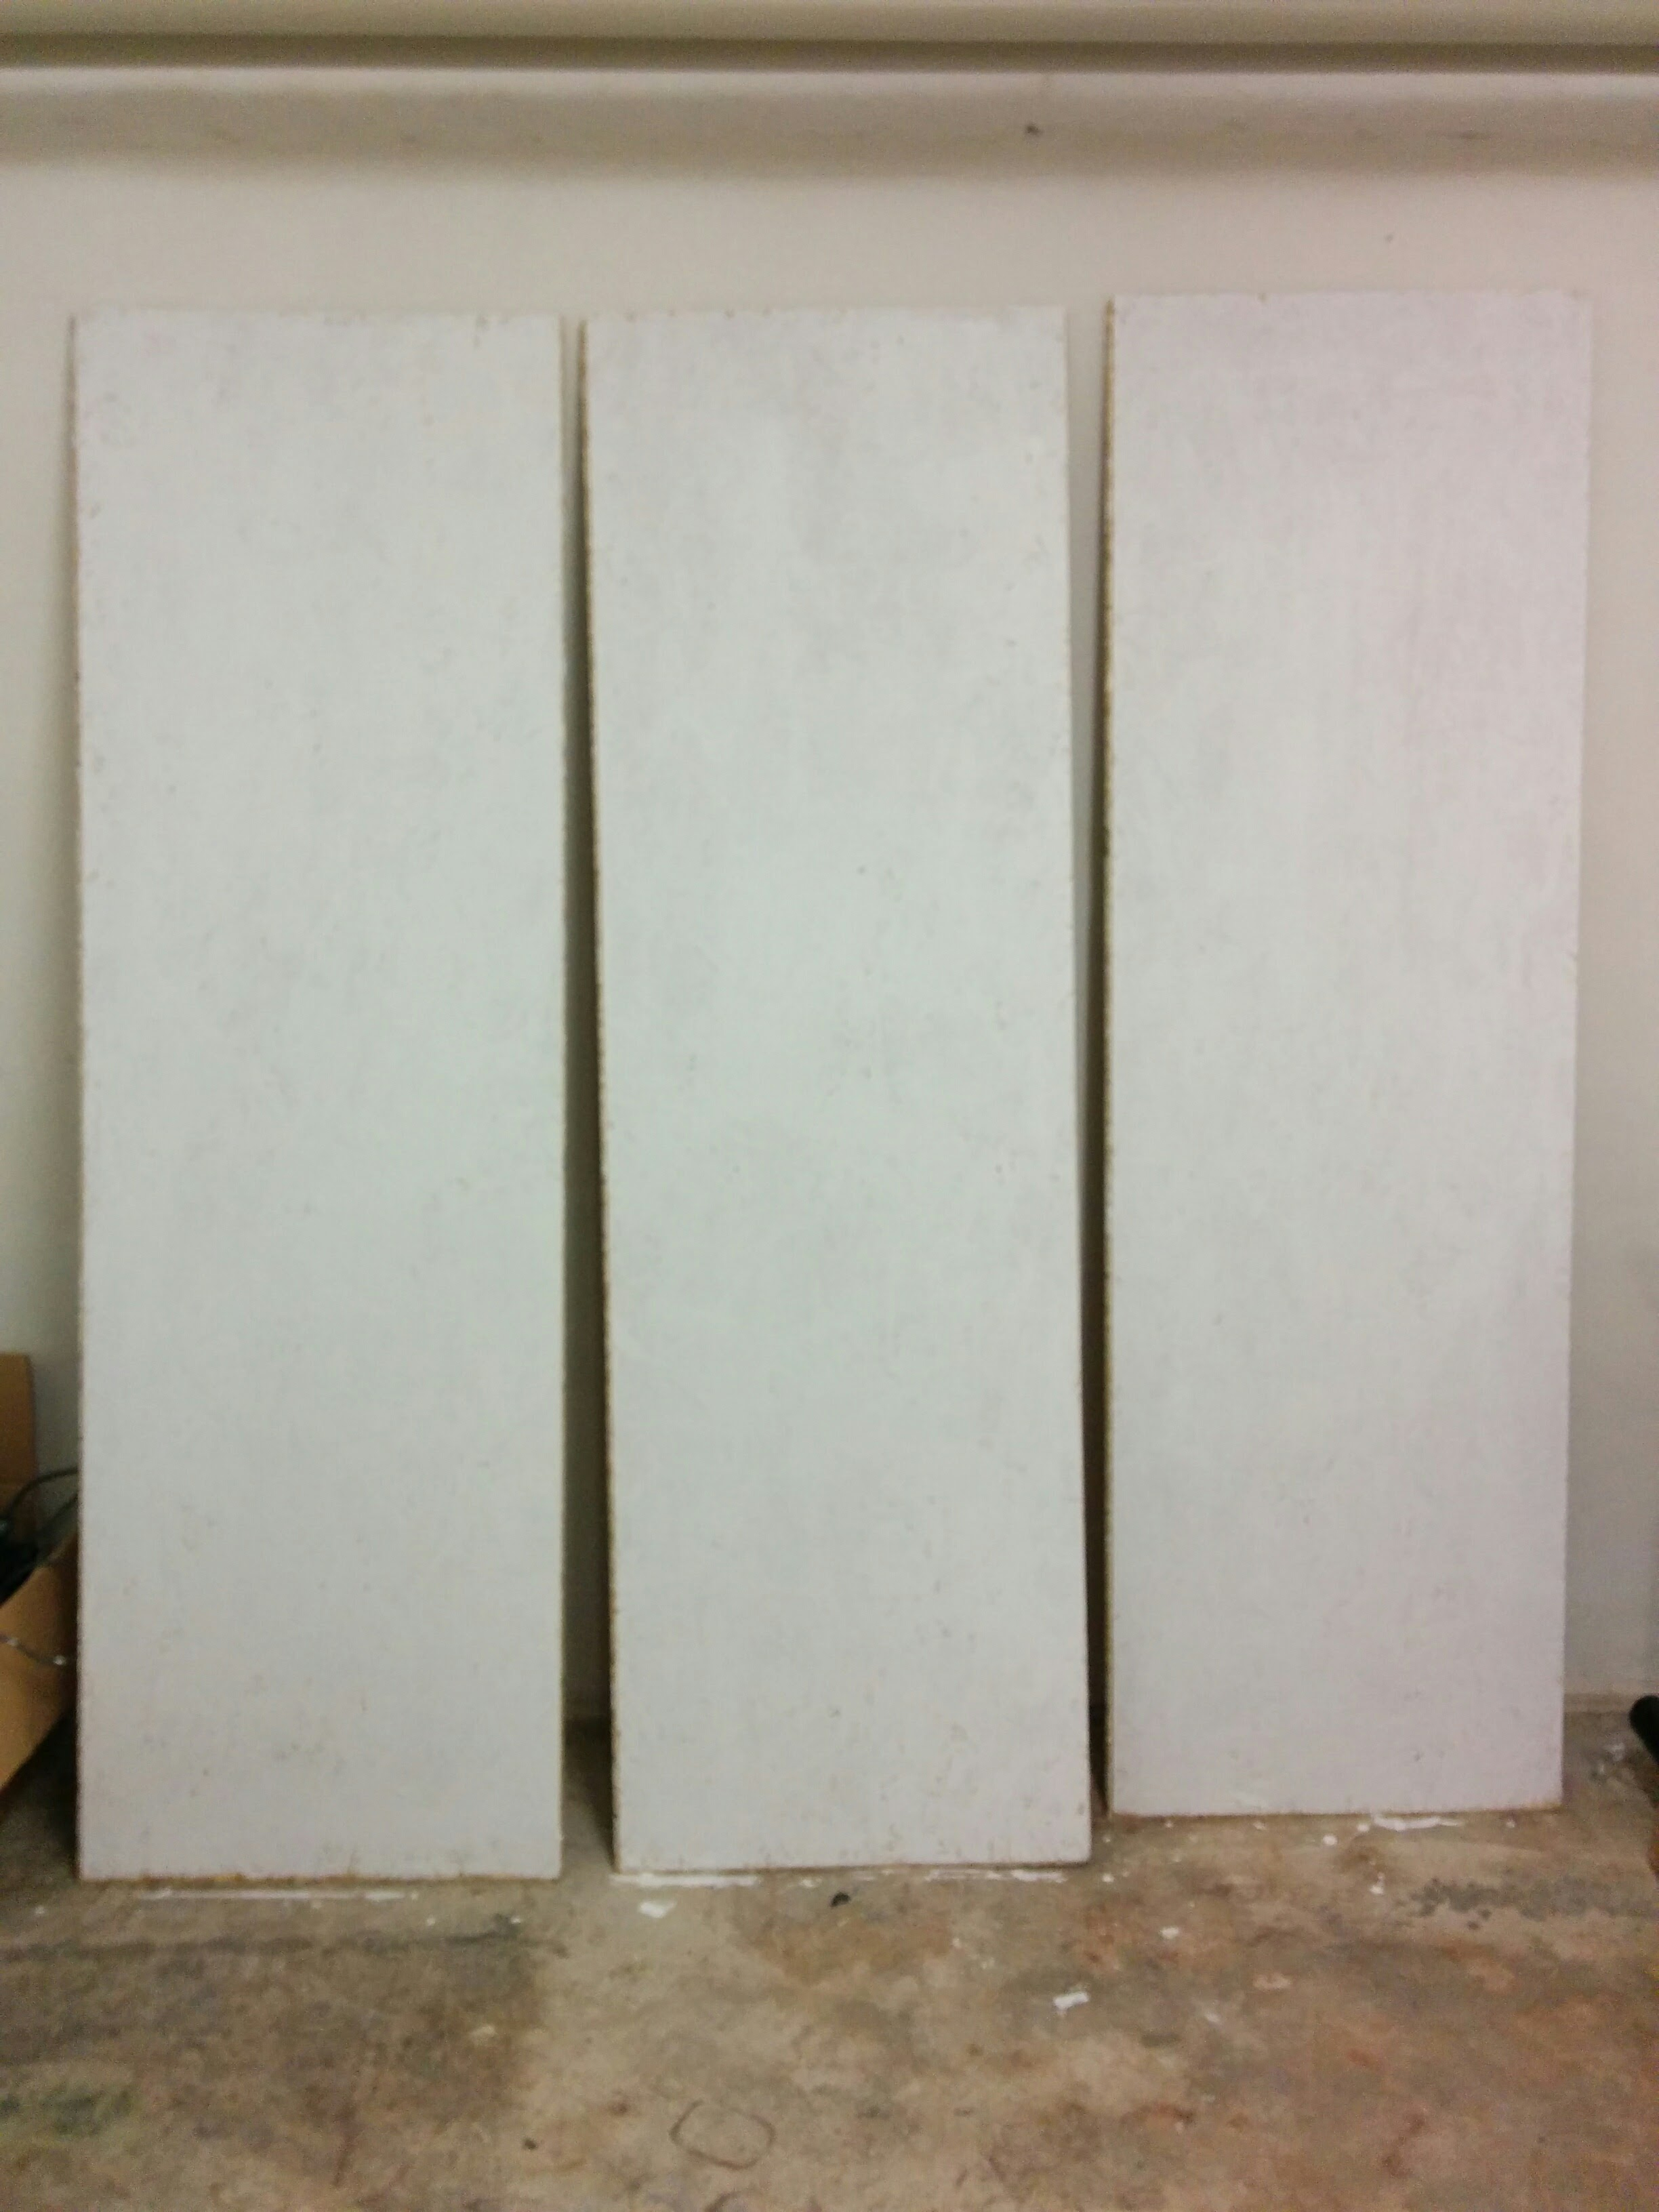
\includegraphics[width=.6\linewidth]{../Bilder/plattenfertig.jpg}
	  \label{fig:sub2}
	\end{subfigure}
	\vspace{10pt}
	\caption{Fertigung der Rennstrecke}
	\label{fig:gebauteStrecke}
	\end{figure}
	
	\subsection{Einführungsrunde}
	
	\subsection{Einbinden der Sensoren}
		
	% Anhang
	\renewcommand{\thetable}{\Alph{section}.\arabic{table}}              % Tabellennummerierung mit Section
	\renewcommand{\thefigure}{\Alph{section}.\arabic{figure}}            % Abbildungsnummerierung mit Section
	\renewcommand{\thelstlisting}{\Alph{section}.\arabic{lstlisting}}    % Listingsnummerierung mit Section
	
	\begin{appendix}
	%\include{chapter/30_anhang}
	\end{appendix}
	
	% Abschluss
	\bibliography{literatur/literatur}
\newpage

	\renewcommand{\indexname}{Stichwortverzeichnis}
\printindex
\newpage

	\thispagestyle{empty}
\addcontentsline{toc}{section}{Selbständigkeitserklärung}
\begin{center}
	\vspace*{2cm}
	\Huge\bf Selbständigkeitserklärung\\
	\vspace*{3cm}
	\normalsize\rm
	Ich versichere hiermit, dass wir unsere \ifcase\myType Studienarbeit \or Projektarbeit \or Bachelorarbeit\else\fi ~mit dem Thema\\
	\vspace*{2cm}
	\Large\bf\myTopic\\
	\vspace*{2cm}
	\normalsize\rm
	selbständig verfasst und keine anderen als die angegebenen\\Quellen und Hilfsmittel benutzt haben.\\
	\bigskip
	\bigskip
	\bigskip
	\bigskip
	\bigskip
	\bigskip
	\bigskip
	\bigskip
	\begin{tabularx}{\textwidth}{l@{\extracolsep\fill}r}
	\rule{7cm}{0.3mm}&\rule{7.55cm}{0.3mm}\\
	\end{tabularx}
	\begin{tabularx}{\textwidth}{*{2}{>{\arraybackslash}X}}
		Ort, Datum&Unterschrift Lara Kroesen\\
	\end{tabularx}
	
	\bigskip
	\bigskip
	\bigskip	
	\begin{tabularx}{\textwidth}{l@{\extracolsep\fill}r}
	\rule{7cm}{0.3mm}&\rule{7.55cm}{0.3mm}\\
	\end{tabularx}
	\begin{tabularx}{\textwidth}{*{2}{>{\arraybackslash}X}}
	  Ort, Datum&Unterschrift Jens Müller\\
	\end{tabularx}
	
	\bigskip
	\bigskip
	\bigskip	
	\begin{tabularx}{\textwidth}{l@{\extracolsep\fill}r}
  	\rule{7cm}{0.3mm}&\rule{7.55cm}{0.3mm}\\
	\end{tabularx}
	\begin{tabularx}{\textwidth}{*{2}{>{\arraybackslash}X}}
	  Ort, Datum&Unterschrift Jan Herkommer\\
	\end{tabularx}
\end{center}

\end{document}

%%%%%%%%%%%%%%%%%%%%%%%%%%%%%%%%%%%%%%%%%%%%%%%%%%%%%%%%%%%%%%%%%%%%%%%%%%%%%
%%                                                                         %%
%% /\   /\         Ab hier keine Änderungen mehr vornehmen         /\   /\ %%
%%                                                                         %%
%%%%%%%%%%%%%%%%%%%%%%%%%%%%%%%%%%%%%%%%%%%%%%%%%%%%%%%%%%%%%%%%%%%%%%%%%%%%%